%%%%%%%%%%%%%%%%%%%%%%%%%%%%%%%%%%%%%%%%%
% Masters/Doctoral Thesis 
% LaTeX Template
% Version 2.3 (25/3/16)
%
% This template has been downloaded from:
% http://www.LaTeXTemplates.com
%
% Version 2.x major modifications by:
% Vel (vel@latextemplates.com)
%
% This template is based on a template by:
% Steve Gunn (http://users.ecs.soton.ac.uk/srg/softwaretools/document/templates/)
% Sunil Patel (http://www.sunilpatel.co.uk/thesis-template/)
%
% Template license:
% CC BY-NC-SA 3.0 (http://creativecommons.org/licenses/by-nc-sa/3.0/)
%
%%%%%%%%%%%%%%%%%%%%%%%%%%%%%%%%%%%%%%%%%

%----------------------------------------------------------------------------------------
%	PACKAGES AND OTHER DOCUMENT CONFIGURATIONS
%----------------------------------------------------------------------------------------

\documentclass[
11pt, % The default document font size, options: 10pt, 11pt, 12pt
%oneside, % Two side (alternating margins) for binding by default, uncomment to switch to one side
%chapterinoneline,% Have the chapter title next to the number in one single line
%english, % ngerman for German
spanish,
singlespacing, % Single line spacing, alternatives: onehalfspacing or doublespacing
%draft, % Uncomment to enable draft mode (no pictures, no links, overfull hboxes indicated)
%nolistspacing, % If the document is onehalfspacing or doublespacing, uncomment this to set spacing in lists to single
%liststotoc, % Uncomment to add the list of figures/tables/etc to the table of contents
%toctotoc, % Uncomment to add the main table of contents to the table of contents
parskip, % Uncomment to add space between paragraphs
%nohyperref, % Uncomment to not load the hyperref package
headsepline, % Uncomment to get a line under the header
]{MastersDoctoralThesis} % The class file specifying the document structure



\usepackage[utf8]{inputenc} % Required for inputting international characters
\usepackage[T1]{fontenc} % Output font encoding for international characters

\usepackage{palatino} % Use the Palatino font by default
%,style=authoryear
\usepackage[backend=bibtex,natbib=true]{biblatex} % Use the bibtex backend with the authoryear citation style (which resembles APA)

\addbibresource{references.bib} % The filename of the bibliography

\usepackage[autostyle=true]{csquotes} % Required to generate language-dependent quotes in the bibliography

\usepackage{caption}
\usepackage{subcaption}

%------------------------
\usepackage{listings}

%\usepackage[hyphens]{url}
%\usepackage[hidelinks]{hyperref}
%\hypersetup{breaklinks=true}
\urlstyle{same}
%\usepackage{cite}

%--------------------------

\usepackage{color}

%
%----------------------------------------------------------------------------------------
%	MARGIN SETTINGS
%----------------------------------------------------------------------------------------

\geometry{
	paper=a4paper, % Change to letterpaper for US letter
	inner=2cm, % Inner margin
	outer=3.3cm, % Outer margin
	bindingoffset=2cm, % Binding offset
	top=1.5cm, % Top margin
	bottom=1.5cm, % Bottom margin
	%showframe,% show how the type block is set on the page
}

%----------------------------------------------------------------------------------------
%	INFORMACIÓN DE LA MEMORIA
%----------------------------------------------------------------------------------------

\thesistitle{Dispositivo Logger IoT con Tecnologías de comunicación Sigfox y Lora} % El títulos de la memoria, se usa en la carátula y se puede usar el cualquier lugar del documento con el comando \ttitle
\supervisor{Ing. Marcelo E. Romeo (UNSAM, UTN-FRBA)} % El nombre del director, se usa en la carátula y se puede usar el cualquier lugar del documento con el comando \supname
\degree{Especialista en Sistemas Embebidos } % Nombre del grado, se usa en la carátula y se puede usar el cualquier lugar del documento con el comando \degreename
\author{Ing. Julian Bustamante Narvaez} % Tu nombre, se usa en la carátula y se puede usar el cualquier lugar del documento con el comando \authorname
\juradoUNO{Esp. Ing. Leonardo carducci (FIUBA)} % Nombre y pertenencia del un jurado se usa en la carátula y se puede usar el cualquier lugar del documento con el comando \jur1name
\juradoDOS{Esp. Ing. Agustin Bassi (FIUBA)} % Nombre y pertenencia del un jurado se usa en la carátula y se puede usar el cualquier lugar del documento con el comando \jur2name
\juradoTRES{Esp. Ing. Ramiro Alonso (FIUBA)} % Nombre y pertenencia del un jurado se usa en la carátula y se puede usar el cualquier lugar del documento con el comando \jur3name
\fechaINICIO{agosto de 2018}
\fechaFINAL{agosto de 2019}

\subject{Memoria del Trabajo Final de la Carrera de Especialización en Sistemas Embebidos de la UBA} % Your subject area, this is not currently used anywhere in the template, print it elsewhere with \subjectname
\keywords{CESE, Sistemas Embebidos, CIAA} % Keywords for your thesis, this is not currently used anywhere in the template, print it elsewhere with \keywordnames
\university{Universidad de Buenos Aires} % Your university's name and URL, this is used in the title page and abstract, print it elsewhere with \univname
\faculty{{Facultad de Ingeniería}} % Your faculty's name and URL, this is used in the title page and abstract, print it elsewhere with \facname
\department{Departamento de Electrónica} % Your department's name and URL, this is used in the title page and abstract, print it elsewhere with \deptname
\group{{Laboratorio de Sistemas Embebidos}} % Your research group's name and URL, this is used in the title page, print it elsewhere with \groupname


\hypersetup{pdftitle=\ttitle} % Set the PDF's title to your title
\hypersetup{pdfauthor=\authorname} % Set the PDF's author to your name
\hypersetup{pdfkeywords=\keywordnames} % Set the PDF's keywords to your keywords


\newcaptionname{spanish}{\acknowledgementname}{Agradecimientos}
\newcaptionname{spanish}{\authorshipname}{Declaración de Autoría}
\newcaptionname{spanish}{\abbrevname}{Glosario}
\newcaptionname{spanish}{\byname}{por}

\renewcommand{\lstlistingname}{Algoritmo}% Listing -> Algorithm
\renewcommand{\lstlistlistingname}{Índice de \lstlistingname s}% List of Listings -> List of Algorithms

\renewcommand{\listtablename}{Índice de Tablas}
\renewcommand{\tablename}{Tabla} 

\addtolength{\footnotesep}{2mm} % Espacio adicional en los footnotes

\begin{document}

\frontmatter % Use roman page numbering style (i, ii, iii, iv...) for the pre-content pages

\pagestyle{plain} % Default to the plain heading style until the thesis style is called for the body content

%----------------------------------------------------------------------------------------
%	CARÁTULA
%----------------------------------------------------------------------------------------

\begin{titlepage}
\begin{center}

{\scshape\LARGE UNIVERSIDAD DE BUENOS AIRES\par}\vspace{0.1cm} % University name
{\scshape\LARGE FACULTAD DE INGENIERÍA\par}\vspace{0.1cm} % Faculty name
{\scshape\LARGE Carrera de Especialización en Sistemas Embebidos\par}\vspace{1cm} % Thesis type


\includegraphics[width=.3\textwidth]{./Figures/logoFIUBA.png}
\vspace{1cm}

\textsc{\Large Memoria del Trabajo Final}\\[0.5cm] % Thesis type

{\huge \bfseries \ttitle\par}\vspace{0.4cm} % Thesis title

\vspace{1cm}
\LARGE\textbf{Autor:\\
\authorname}\\ % Author name

\vspace{1cm}

\large
\vspace{10px}
{Director:} \\
{\supname} % Supervisor name
 
\vspace{1cm}
Jurados:\\
\jurunoname\\
\jurdosname\\
\jurtresname
 
\vfill
\textit{Este trabajo fue realizado en las Ciudad Autónoma de Buenos Aires, entre \fechaINICIOname \hspace{1px} y \fechaFINALname.}
\end{center}
\end{titlepage}


%----------------------------------------------------------------------------------------
%	RESUMEN - ABSTRACT 
%----------------------------------------------------------------------------------------

\begin{abstract}
\addchaptertocentry{\abstractname} % Add the abstract to the table of contents
%
%The Thesis Abstract is written here (and usually kept to just this page). The page is kept centered vertically so can expand into the blank space above the title too\ldots
\centering

Este proyecto consistió en diseñar e implementar un dispositivo de adquisición de datos con múltiples entradas digitales y análogicas para aplicaciones IoT en ambientes industriales
para la empresa Tecrea S.A.S. El dispositivo tiene una arquitectura modular que le permite incorporar nuevas funcionalidades y puede operar con protocolos
inalámbricos como SigFox y Lora.

La importancia de este proyecto se enfocó en que los procesos sean menos dependientes de las personas y que se puedan auto gestionar con información
adquirida en tiempo real.

En la presente memoria se plasman los conocimientos adquiridos en la carrera, mejorando la metodología actual en el desarrollo de firmware en sistemas embebidos, 
testing de software, diseño electrónico, circuitos impresos y gestión de proyectos.

\end{abstract}

%----------------------------------------------------------------------------------------
%	CONTENIDO DE LA MEMORIA  - AGRADECIMIENTOS
%----------------------------------------------------------------------------------------

\begin{acknowledgements}
%\addchaptertocentry{\acknowledgementname} % Descomentando esta línea se puede agregar los agradecimientos al índice
\vspace{1.5cm}

Agradecimientos personales. \textbf{[OPCIONAL]} 

No olvidarse de agradecer al tutor.

No vale poner anti-agradecimientos (este trabajo fue posible a pesar de...)

\end{acknowledgements}

%----------------------------------------------------------------------------------------
%	LISTA DE CONTENIDOS/FIGURAS/TABLAS
%----------------------------------------------------------------------------------------
\renewcommand{\listtablename}{Índice de Tablas}

\tableofcontents % Prints the main table of contents

\listoffigures % Prints the list of figures

\listoftables % Prints the list of tables


%----------------------------------------------------------------------------------------
%	CONTENIDO DE LA MEMORIA  - DEDICATORIA
%----------------------------------------------------------------------------------------

\dedicatory{\textbf{Dedicado a... [OPCIONAL]}}  % escribir acá si se desea una dedicatoria

%----------------------------------------------------------------------------------------
%	CONTENIDO DE LA MEMORIA  - CAPÍTULOS
%----------------------------------------------------------------------------------------

\mainmatter % Begin numeric (1,2,3...) page numbering

\pagestyle{thesis} % Return the page headers back to the "thesis" style

\renewcommand{\tablename}{Tabla} 

% Incluir los capítulos como archivos separados desde la carpeta Chapters
% Descomentar las líneas a medida que se escriben los capítulos

% Chapter 1

\chapter{Introducción General} % Main chapter title
En este capítulo se menciona la problematica que motivó la realización del presente trabajo, los procedimientos de la toma de datos en la industría actualmente y el enfoque elegido para desarrollar el prototipo que ofrece una solución usando sistemas embebidos.
\label{Chapter1} % For referencing the chapter elsewhere, use \ref{Chapter1} 
\label{IntroGeneral}

%----------------------------------------------------------------------------------------

% Define some commands to keep the formatting separated from the content 
\newcommand{\keyword}[1]{\textbf{#1}}
\newcommand{\tabhead}[1]{\textbf{#1}}
\newcommand{\code}[1]{\texttt{#1}}
\newcommand{\file}[1]{\texttt{\bfseries#1}}
\newcommand{\option}[1]{\texttt{\itshape#1}}
\newcommand{\grados}{$^{\circ}$}

%----------------------------------------------------------------------------------------

%\section{Introducción}

%----------------------------------------------------------------------------------------
\section{Motivación}
En el transcurso de la próxima década se espera un gran crecimiento en la cantidad de dispositivos IoT (\textit{internet of things}) provenientes de redes LPWAN (\textit{Low-Power Wide Area Network}). Para el 2025, se espera que más de 100 billones de dispositivos se conecten a través de LPWAN\cite{taylor2015world}. Las principales tecnologías, que prometen una vida útil alta de la batería de los dispositivos y un alcance de hasta 15 kilómetros, son Sigfox, Lora y NB-IoT, que actualmente están conectados en todo el mundo con más de 25 millones de dispositivos, brindando servicio y facilitando las experiencias del usuario\cite{iotanalytics}.

En los procesos industriales se tiene mucha información de variables físicas y eléctricas por medio de sensores, la cual muchas veces no se aprovecha debido a que no se tiene una óptima trazabilidad de la misma o simplemente se pierde esta información. Cuando los procesos industriales fallan, necesitan una reacción inmediata por parte de una persona y esto genera una dependencia de alguien que no siempre va a estar las 24 horas del día al pendiente, quizá por costos para las mismas empresas.

En vista de lo de anterior se desarrolló un prototipo para ofrecer una solución que permita monitorear inalambricamente diferentes variables en los procesos industriales de esta manera los usuarios pueden estar informados y garantizan la correcta funcionalidad de sus procesos.

%https://iot-analytics.com/state-of-the-iot-update-q1-q2-2018-number-of-iot-devices-now-7b/


\section{IoT (\textit{Internet of Things})}
El concepto de internet de las cosas se refiere a la interconexión digital de dispositivos y objetos  a través  de una red, es decir, dispositivos como sensores y/o actuadores, equipados con una interfaz de comunicación, unidades de procesamiento y almacenamiento\cite{centenaro2016long}. Estos dispositivos tienen la capacidad de adquirir, intercambiar y transferir datos a la red mediante alguna tecnología de comunicación inalámbrica.



IoT es una tendencia imparable y puede facilitar mucho la vida diaria. Produce formas baratas y efectivas de resolver grandes problemas sociales, como el acceso a la energía, el transporte y la vivienda. Otras aplicaciones pueden ser \textit{wearables}, construcciones y demóticas, \textit{smart cities}, \textit{smart manufacturing}\citep{taylor2015world}. IoT puede hacernos sentir más cómodos en nuestros hogares y en nuestras ciudades.

\subsection{Tecnologías de comunicación}
Uno de los principales habilitadores de un proyecto de internet de las cosas son las redes de comunicaciones. Estas permiten conectar dispositivos, máquinas, sensores o “cosas” los cuales generan datos o información desde cualquier punto geográfico del planeta. Las redes de comunicación son un conjunto de medios técnicos que permiten la comunicación entre equipos que se encuentran a distancia.

Las principales características de una red de comunicación IoT son:
\begin{itemize}
	\item Baja tasa de datos.
	\item Bajo consumo de energía.
	\item Largo alcance de comunicación.
	\item Conexiones bidireccionales.
	\item Movilidad y servicios de localización.

\end{itemize}

En la tabla \ref{tab:Tecno} se puede observar una comparación de las principales tecnologías de comunicación.

\begin{table}[h]
	\centering
	\caption[Redes de comunicación]{Redes de comunicación más utilizadas para proyectos IoT}
	\begin{tabular}{l c c c}    
		\toprule
		\textbf{Tecnología} 	 & \textbf{Consumo}  & \textbf{Alcance} 	& \textbf{Tasa de Datos} \\
		\midrule
		GSM/GPRS				 & Muy alto			& Alto					&	Alta \\		
		SigFox					 & Bajo				& Medio/alto			&	Muy baja \\
		Lora					 & Bajo				& Medio/alto			&	Muy baja\\	
		WiFi					 & Alto				& Bajo					&	Muy alta \\
		BLE					 	 & Muy bajo			& Muy Bajo				&	Baja \\
		ZigBee					 & Medio			& Bajo					&	Baja \\	
		\bottomrule
		\hline
	\end{tabular}
	\label{tab:Tecno}
\end{table}

\textbf{Tecnología GSM/GPRS:}

GSM (\textit{Global System for Mobile communications)} o en español sistema global para las comunicaciones móviles y es un tipo de red que se utiliza para la transmisión móvil de voz y datos.

GPRS (\textit{General Packet Radio Service)} o en español servicio general de paquetes vía radio y es una extensión mejorada del GSM.
Permite la mensajería instantánea, los servicios de mensajes cortos SMS (\textit{Short Message Service}), multimedia MMS (\textit{Multimedia Messaging Service}) y correo electrónico. Esta proporciona una cobertura inalámbrica completa, tiempos de acceso mas cortos y mayores tasas de datos\citep{bettstetter1999gsm}. Por ejemplo, permite enviar 30 SMS por minuto, mientras que con GSM se puede enviar entre 6 y 10.

\textbf{Tecnología WiFi:}

Es una tecnología que permite la interconexión inalámbrica de dispositivos electrónicos por medio de internet. WiFi, el nombre popular para el área local inalámbrica Redes basadas en el estándar IEEE 802.11b, se ha convertido en la Tecnología preferida para redes inalámbricas de área local en entornos comerciales y domésticos\citep{henry2002wifi}.

\textbf{Tecnología BLE:}

Es una tecnología de red de área personal PAN (\textit{Personal Area Network}) inalámbrica, Permite la comunicación entre dispositivos dos o  más dispositivos Bluetooth, que opera en 2.4 GHz (una de las bandas ISM), con una tasa de transferencia de 1 Mbps en la capa física. BLE (\textit{Bluetooth Low Energy}) se introdujo por primera vez en 2010 con el objetivo de expandir la aplicación de Bluetooth para su uso en dispositivos con limitaciones de energía, como los inalámbricos. Sensores y controles inalámbricos. Los sensores y controles requieren un bajo consumo de energía, pero la cantidad de transmisión de datos es pequeña y la comunicación ocurre con poca frecuencia\citep{chang2014bluetooth}.


\textbf{Tecnología ZigBee:}

ZigBee es uno de El transceptor estándar más utilizado en sensores inalámbricos.redes ZigBee sobre IEEE 802.15.4 , define especificaciones para baja velocidad de datos WPAN (\textit{wireless personal area network}) para soportar baja potencia en monitorización y control de dispositivos\citep{ramya2011study}.

El consumo de energía para ZigBee es muy pequeño. En la mayoría de los casos Utiliza 1mW (o menos potencia). Pero aún así proporciona un alcance hasta 150 metros en exterior que se consigue con la técnica.llamado espectro de propagación de secuencia directa DSSS (\textit{direct sequence spread spectrum}).Funciona en los 868 MHz (Europa), 915 MHz (América del Norte y Australia) y 2.4 GHz (disponible en todo el mundo) banda ISM con hasta 20kbps, 40kbps y velocidad de datos de 250kbps respectivamente\citep{ramya2011study}.

\textbf{Tecnología NB-IoT (\textit{Narrowband Internet of Things}:}

Tecnología de acceso por radio que proporciona cobertura extendida, alta capacidad y larga duración de la batería. Utiliza la ya existente red móvil para conectar dispositivos de manera masiva.

NB-IoT requiere un ancho de banda mínimo de 180 kHz, que es igual al tamaño del LTE físico más pequeño.
Dependiendo de la disponibilidad del espectro, esta tecnología se puede implementar por sí solo en los portadores de guardia de LTE / UMTS existentes\citep{adhikary2016performance}.

\textbf{Tecnología LTE-M:}

Es un tipo de tecnología de radio de red LPWAN que permite una amplia gama de dispositivos celulares y servicios (específicamente, para aplicaciones de máquina a máquina e IoT). Utiliza la ya existente red móvil para conectar dispositivos de manera masiva.

\textbf{Tecnología SigFox:} 

Es una tecnología de comunicación UNB (\textit{Ultra-Narrow Band}) para conectar sensores y dispositivos. Opera en las bandas 868 MHz y 902-928 MHz.

\textbf{Tecnología LoRa:} 

Es una tecnología LPWAN de modulación de radio de CCS (\textit{chirp spread spectrum}). Esta permite el envió y recepción de información en las bandas de frecuencia 433 MHz, 868 MHZ y 915 MHz .

%---------------Objetivos y alcance 
\section{Objetivos y alcance}

\subsection{Objetivo}
El objetivo principal es diseñar e implementar un dispositivo de adquisición de datos con múltiples entradas digitales y analógicas para aplicaciones IoT en ambientes industriales, mediante la transmisión inalámbrica de la información por medio de tecnologías de comunicación Sigfox o Lora. 

\subsection{Alcance}

En la presente solución se contempla:


\begin{itemize}
	\item La implementación de un prototipo funcional de hardware.
	\item 2 entradas analógicas de tensión.
	\item 1 entrada analógica de corriente.
	\item 5 entradas digitales.
	\item La escritura del firmware del dispositivo.
	\item La transmisión de la información por medio de Sigfox.
	\item La transmisión de la información por medio de Lora.
	\item La visualización de la información en una plataforma paga o libre.
	\item Se incluye partes del código de la biblioteca usada para el modulo Sigfox.
\end{itemize}
En la presente solución no se contempla:
\begin{itemize}
	\item El desarrollo de la plataforma web que permite visualizar los datos en linea.
	\item Caja plástica del dispositivo.
\end{itemize}
En la presente solución no se incluye:
\begin{itemize}
	\item Diagramas esquemáticos.
	\item PCB \textit{layout}.
	\item Firmware.
\end{itemize}

Esto debido a que la propiedad intelectual es de Tecrea SAS.


%----------------------------------------------------------------------------------------


\chapter{Introducción Específica} % Main chapter title

\label{Chapter2}

%----------------------------------------------------------------------------------------
%	SECTION 1
%----------------------------------------------------------------------------------------
En este capitulo se muestra la idea general del proyecto y se describen las características principales de la solución implementada.
\section{Estructura general del sistema}

%\label{sec:ejemplo}

El diagrama general del sistema se muestra en figura \ref{fig:esquemaGeneral}. El sistema se compone de un microcontrolador ARM(\textit{Advanced RISC Machine}) Cortex\textregistered -M4 y dos bus UART(\textit{Universal Asynchronous Receiver-Transmitter}) para que el sistema pueda tener una arquitectura modular que le permite incorporar nuevas tecnologías de comunicación para transmitir inalambricamente tales como: SigFox, LoRa, Nb-IOT, Cat-M, WiFi y 3G.


\begin{figure}[h]

	\centering

	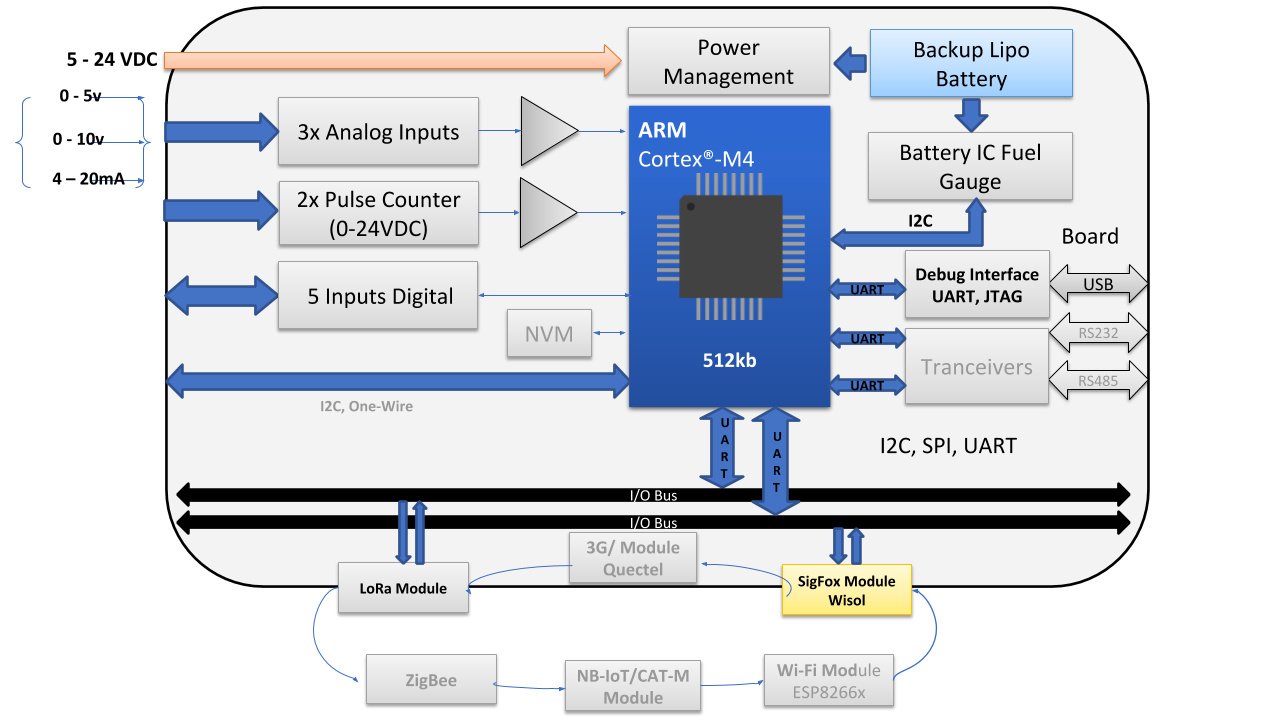
\includegraphics[scale=.35]{./Figures/esquemaGeneral.png}

	\caption{Diagrama general del sistema.}

	\label{fig:esquemaGeneral}

\end{figure}


El sistema consta de un medidor de voltaje para batería de LiPo, dos entradas analógicas de tensión, una de corriente y cinco entradas digitales con el fin de poder adquirir datos de diferentes variables en los procesos industriales. El dispositivo esta diseñado para tener diferentes funcionalidades sin embargo debido a la delimitación del alcance del trabajo no se tubo en cuenta los subsitemas que se observan en gris en la figura \ref{fig:esquemaGeneral}.


\section{Requerimientos}
Los siguientes son los requerimientos del presente trabajo:

\textbf{Grupo de requerimientos asociados al hardware:}
\begin{enumerate}

	\item Microcontrolador.

	\begin{itemize}

		\item Debe tener procesador ARM Cortex M0+ o M4.

		\item Debe tener 3 puertos UART.

		\item Debe tener comunicación I2C/SPI.

		\item Debe tener memoria flash mayor a 64 kb.

		\item Debe tener 3 entradas analógicas.

		\item Debe tener 5 entradas digitales.

	\end{itemize}

	%\item Nivel de protección debe ser IP65.

	\item Autonomía de la batería debe ser de 1 días.

	\item Módulo Sigfox.

		\begin{itemize}

			\item Debe tener un módulo Dual Zone con comunicación por UART.

			\item Debe tener antena externa con centro de banda en 915 MHz.

		\end{itemize}

	\item Módulo Lora.

		\begin{itemize}

			\item Debe tener un módulo con comunicación por UART/I2C.

			\item Debe tener antena externa con centro de banda en 915 MHz.

		\end{itemize}

		\item El sistema debe tener una (1) entrada analógica de voltaje de 0-5 Vdc.
		
		\item El sistema debe tener una (1) entrada analógica de voltaje de 0-10 Vdc.

		\item El sistema debe tener una (1) entradas analógicas de corriente 4-20 mA.

		\item El sistema debe tener cinco (5) entradas digitales 3.3-24 Vdc.

\end{enumerate}



\textbf{Grupo de requerimientos asociados al módulo Sigfox:}

	\begin{enumerate}

		\item Debe colocarse en modo de bajo consumo mientras no esté en uso.

		\item Transmisiones Uplink al backend de sigfox máximo 50 mensajes por día.

		\item Verificación de cada respuesta de comando AT enviado desde el MCU al módulo SIgFox.

	\end{enumerate}





\textbf{Grupo de requerimientos asociados al módulo Lora:}

	\begin{enumerate}

		\item Verificación de cada respuesta de los comandos enviados desde el MCU al módulo Lora.

		\item Debe colocarse en modo de bajo consumo mientras no esté en uso.

	\end{enumerate}



\textbf{Otros requerimientos:}

\begin{enumerate}

	\item En el sistema se podrán configurar umbrales máximos y mínimos de las lecturas analógicas.

	\item El sistema deberá verificar las entradas analógicas cada 1 minuto (parámetro configurable).

	\item El sistema saldrá del modo de bajo consumo cada vez que ocurra una interrupción externa.

\end{enumerate}



\subsection{Sigfox}
Contexto y explicación  completo de que es Sigfox...
Contexto y explicación  completo de que es Sigfox...
Contexto y explicación  completo de que es Sigfox...
\subsection{Lora}
Contexto y explicacióncompleto de que es Lora...

%\section{Antecedentes}

Si se desea indicar alguna página web utilizar el siguiente formato de referencias bibliográficas, dónde las referencias se detallan en la sección de bibliografía de la memoria,utilizado el formato establecido por IEEE en \citep{IEEE:citation}. Por ejemplo, ``el presente trabajo se basa en la plataforma EDU-CIAA-NXP, la cual se describe en detalle en \citep{CIAA}''.

\subsection{Figuras} 

La forma correcta de utilizar una figura es la siguiente: ``Se eligió utilizar un cuadrado azul para el logo, el cual se ilustra en la figura \ref{fig:esquemaGeneral}''.

%\begin{figure}[h]
%	\centering
%	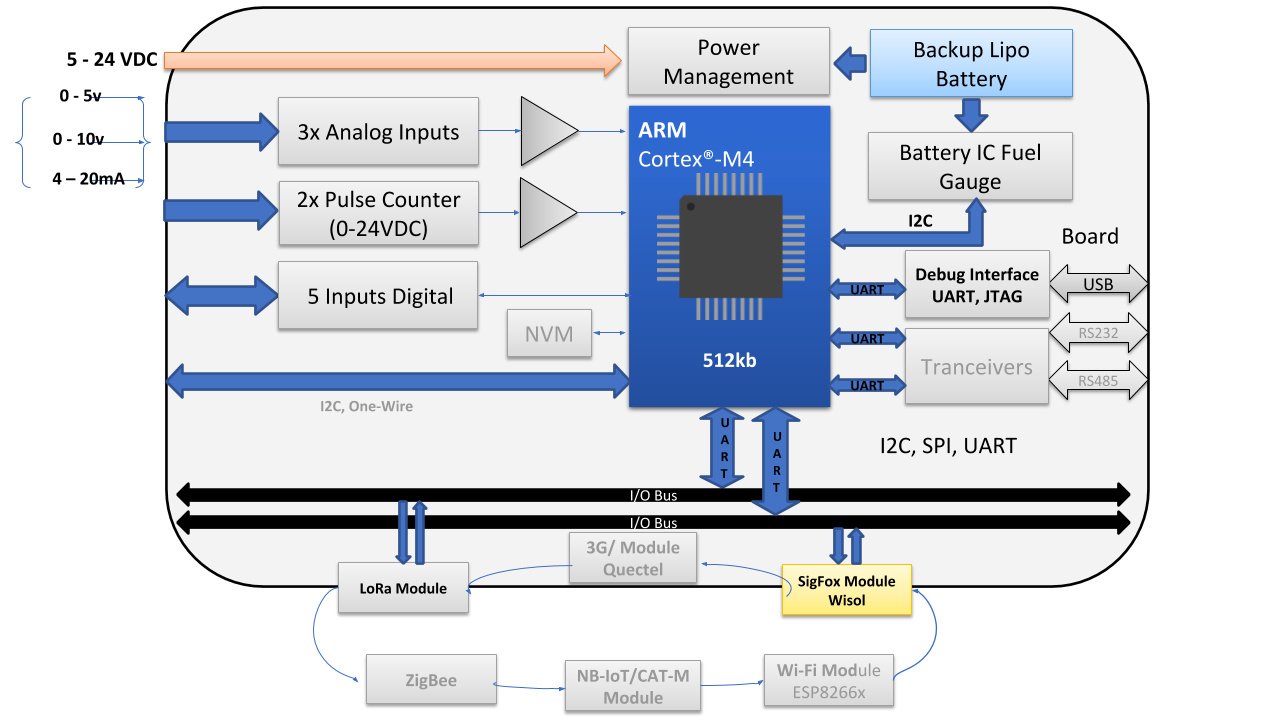
\includegraphics[scale=.35]{./Figures/esquemaGeneral.png}
%	\caption{Diagrama general del sistema.}
%	\label{fig:esquemaGeneral}
%\end{figure}

El texto de las figuras debe estar siempre en español, excepto que se decida reproducir una figura original tomada de alguna referencia. En ese caso la referencia de la cual se tomó la figura debe ser indicada en el epígrafe de la figura e incluida como una nota al pie, como se ilustra en la figura \ref{fig:palabraIngles}.

\begin{figure}[h!]
	\centering
	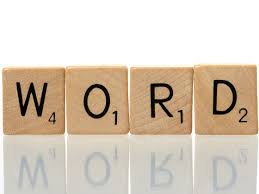
\includegraphics[scale=.25]{./Figures/word.jpeg}
	\caption{Imagen tomada de la página oficial del procesador\protect\footnotemark.}
	\label{fig:palabraIngles}
\end{figure}

\footnotetext{\url{https://goo.gl/images/i7C70w}}


La figura y el epígrafe deben conformar una unidad cuyo significado principal pueda ser comprendido por el lector sin necesidad de leer el cuerpo central de la memoria. Para eso es necesario que el epígrafe sea todo lo detallado que corresponda y si en la figura se utilizan abreviaturas entonces aclarar su significado en el epígrafe o en la misma figura.

\begin{figure}[h]
	\centering
	
\includegraphics[scale=.4]{./Figures/questionMark.png}
	\caption{El lector no sabe por qué de pronto aparece esta figura.}
	\label{fig:questionMark}
\end{figure}

Nunca colocar una figura en el documento antes de hacer la primera referencia a ella, como se ilustra con la figura \ref{fig:questionMark}, porque sino el lector no comprenderá por qué de pronto aparece la figura en el documento, lo que distraerá su atención.

\subsection{Ecuaciones}
\label{sec:Ecuaciones}

Al insertar ecuaciones en la memoria estas se deben numerar de la siguiente forma:

\begin{equation}
	\label{eq:metric}
	ds^2 = c^2 dt^2 \left( \frac{d\sigma^2}{1-k\sigma^2} + \sigma^2\left[ d\theta^2 + \sin^2\theta d\phi^2 \right] \right)
\end{equation}
                                                        
Es importante tener presente que en el caso de las ecuaciones estas pueden ser referidas por su número, como por ejemplo ``tal como describe la ecuación \ref{eq:metric}'', pero también es correcto utilizar los dos puntos, como por ejemplo ``la expresión matemática que describe este comportamiento es la siguiente:''

\begin{equation}
	\label{eq:schrodinger}
	\frac{\hbar^2}{2m}\nabla^2\Psi + V(\mathbf{r})\Psi = -i\hbar \frac{\partial\Psi}{\partial t}
\end{equation}

Para las ecuaciones se debe utilizar un tamaño de letra equivalente al utilizado para el texto del trabajo, en tipografía cursiva y preferentemente del tipo Times New Roman o similar. El espaciado antes y después de cada ecuación es de aproximadamente el doble que entre párrafos consecutivos del cuerpo principal del texto. Por suerte la plantilla se encarga de esto por nosotros.

Para generar la ecuación \ref{eq:metric} se utilizó el siguiente código:

\begin{verbatim}
\begin{equation}
	\label{eq:metric}
	ds^2 = c^2 dt^2 \left( \frac{d\sigma^2}{1-k\sigma^2} + 
	\sigma^2\left[ d\theta^2 + 
	\sin^2\theta d\phi^2 \right] \right)
\end{equation}
\end{verbatim}

Y para la ecuación \ref{eq:schrodinger}:

\begin{verbatim}
\begin{equation}
	\label{eq:schrodinger}
	\frac{\hbar^2}{2m}\nabla^2\Psi + V(\mathbf{r})\Psi = 
	-i\hbar \frac{\partial\Psi}{\partial t}
\end{equation}

\end{verbatim} 
\chapter{Diseño e Implementación} % Main chapter title

\label{Chapter3} % Change X to a consecutive number; for referencing this chapter elsewhere, use \ref{ChapterX}
\definecolor{mygreen}{rgb}{0,0.6,0}
\definecolor{mygray}{rgb}{0.5,0.5,0.5}
\definecolor{mymauve}{rgb}{0.58,0,0.82}

\lstset{ %
  backgroundcolor=\color{white},   % choose the background color; you must add \usepackage{color} or \usepackage{xcolor}
  basicstyle=\footnotesize,        % the size of the fonts that are used for the code
  breakatwhitespace=false,         % sets if automatic breaks should only happen at whitespace
  breaklines=true,                 % sets automatic line breaking
  captionpos=b,                    % sets the caption-position to bottom
  commentstyle=\color{mygreen},    % comment style
  deletekeywords={...},            % if you want to delete keywords from the given language
  %escapeinside={\%*}{*)},          % if you want to add LaTeX within your code
  %extendedchars=true,              % lets you use non-ASCII characters; for 8-bits encodings only, does not work with UTF-8
  %frame=single,	                   % adds a frame around the code
  keepspaces=true,                 % keeps spaces in text, useful for keeping indentation of code (possibly needs columns=flexible)
  keywordstyle=\color{blue},       % keyword style
  language=[ANSI]C,					% the language of the code
  %otherkeywords={*,...},           % if you want to add more keywords to the set
  numbers=left,                    % where to put the line-numbers; possible values are (none, left, right)
  numbersep=5pt,                   % how far the line-numbers are from the code
  numberstyle=\tiny\color{mygray}, % the style that is used for the line-numbers
  rulecolor=\color{black},         % if not set, the frame-color may be changed on line-breaks within not-black text (e.g. comments (green here))
  showspaces=false,                % show spaces everywhere adding particular underscores; it overrides 'showstringspaces'
  showstringspaces=false,          % underline spaces within strings only
  showtabs=false,                  % show tabs within strings adding particular underscores
  stepnumber=1,                    % the step between two line-numbers. If it's 1, each line will be numbered
  stringstyle=\color{mymauve},     % string literal style
  tabsize=2,	                   % sets default tabsize to 2 spaces
  title=\lstname,                   % show the filename of files included with \lstinputlisting; also try caption instead of title
  morecomment=[s]{/*}{*/}%
}


%----------------------------------------------------------------------------------------
%	SECTION 1
%----------------------------------------------------------------------------------------
\section{Módulos del sistema de hardware}
 
En el presente capitulo se realiza una explicación detallada de los módulos del hardware, tecnologías usadas, y el diseño e implementación del firmware.


\subsection{Hardware}

En esta sección se explican todos los módulos de hardware que componen el prototipo del proyecto.

En la figura \ref{fig:Hierarchy} se puede observar la jerarquia del diagrama esquemático de todo el hardware.

\begin{figure}[h]
	\centering
	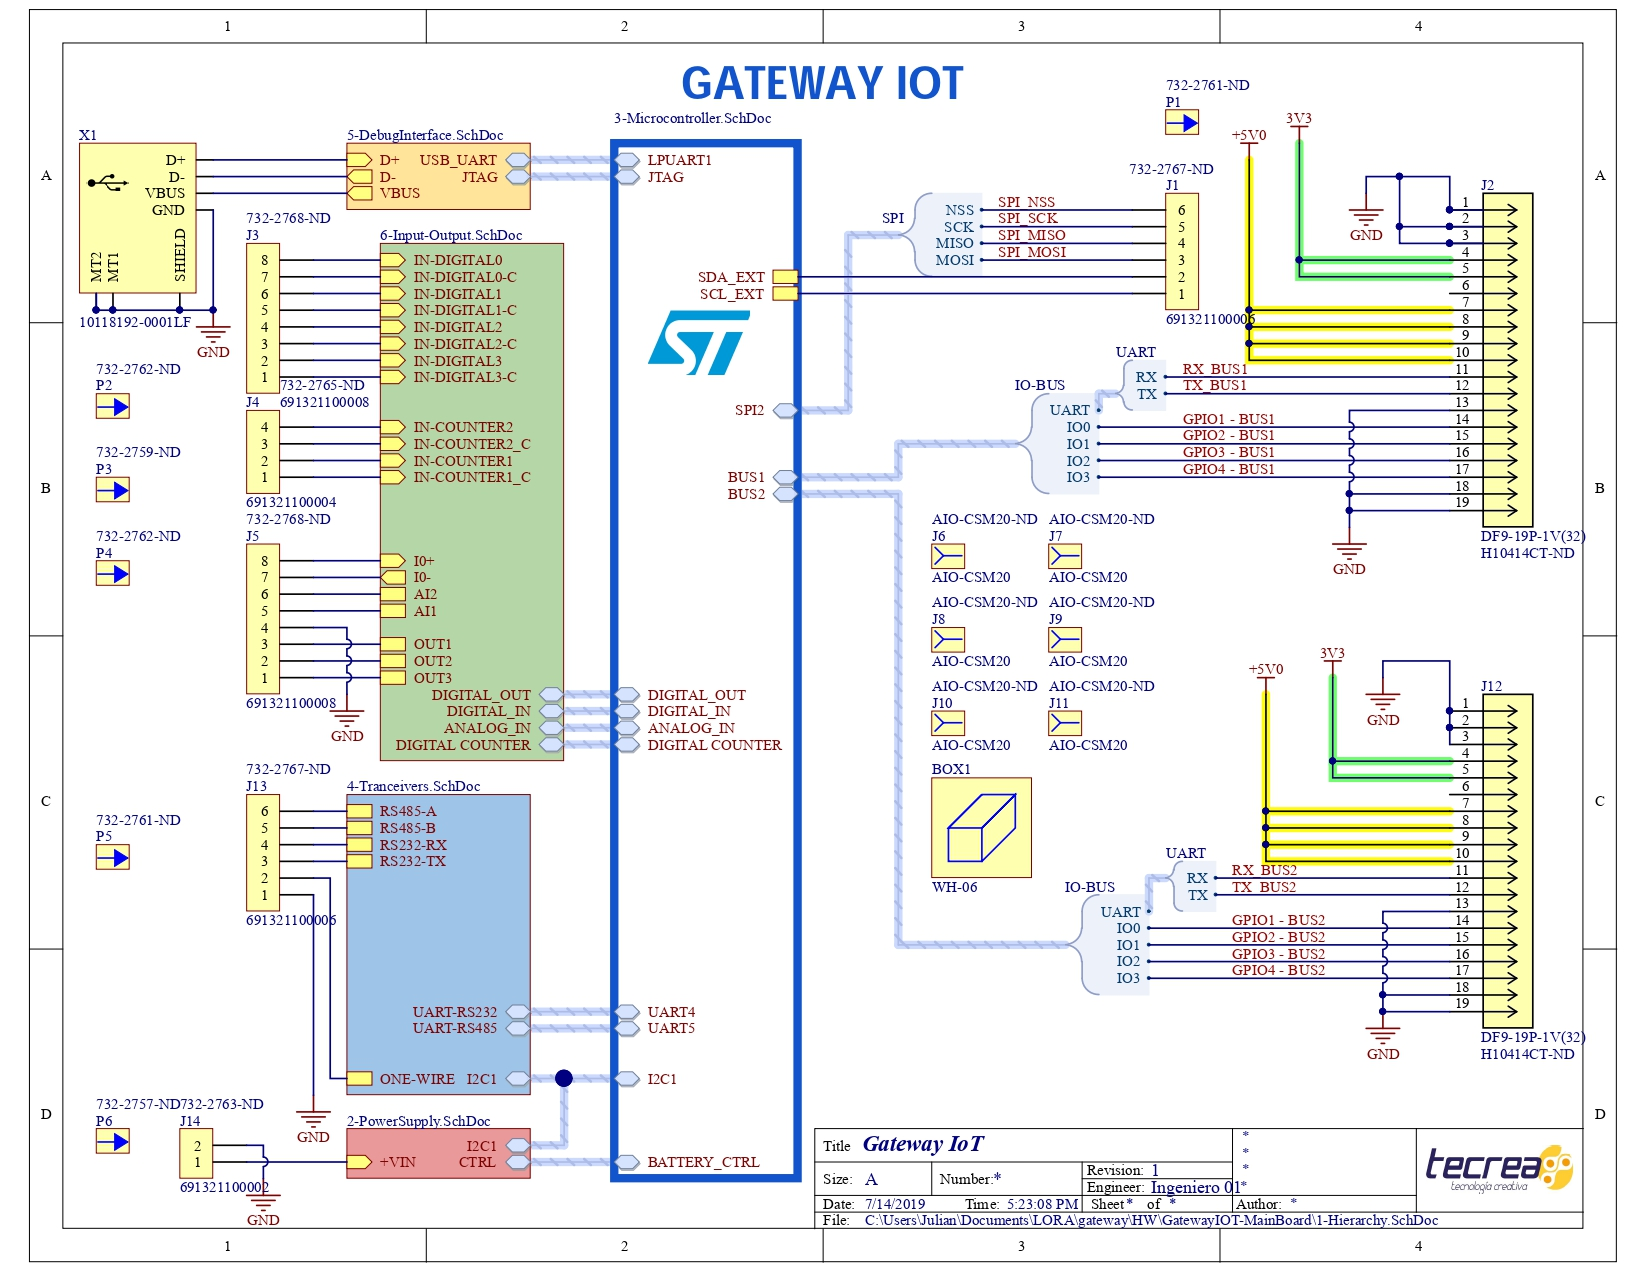
\includegraphics[scale=.6]{./Figures/Hierarchy.jpg}
	\caption{Jerarquia del hardware.}
	\label{fig:Hierarchy}
\end{figure}

\subsubsection{Microcontrolador:}

\begin{itemize}
    \item \textit{Ultra low power} ARM Cortex\textregistered-M4  CPU with FPU
    \item  SRAM 256 KB
    \item 30 nA \textit{Shutdown mode (5 wakeup pins)}
    \item 120 nA \textit{Standby mode (5 wakeup pins)}
    \item 420 nA \textit{Standby mode with RTC}
   \item 3x I2C FM+(1 Mbit/s), SMBus/PMBus 
   \item 6x USARTs
   \item 3x SPIs
   \item 14-\textit{channel DMA controller}
    \item 16 x \textit{ timers}: 2 x 16-bit \textit{advanced motor-control}, 2 x 32-bit and 5 x 16-bit \textit{general purpose}, 2x 16-bit \textit{basic}, 2x \textit{low-power} 16-bit \textit{timers (available in Stop mode)}, 2x \textit{watchdogs, SysTick timer}
    \item \textit{Up to 114 fast I/Os, most 5 V-tolerant, up to 14 I/Os with independent supply down to 1.08 V}
\end{itemize}



\subsubsection{Modulo Sigfox}
El módulo para la comunicación Sigfox desarrollado por la empresa WISOL, opera en 2 zonas con frecuencia distinta, la cual puede ser configurable por software.
\begin{itemize}
    \item WISOL WSSFM11R2D \protect\footnotemark
    \item \textit{RF Frecuency} RC2 transmisión 902.2 MHz.
    \item \textit{RF Frecuency} RC2 recepción 905.2 MHz.
    \item \textit{RF Frecuency} RC4 transmisión 920.8 MHz.
    \item \textit{RF Frecuency} RC4 recepción 922.3 MHz.
    \item potencia de Transmisión 22.5 dBm.
    \item 2.5 uA en modo \textit{sleep}.
\end{itemize}
\footnotetext{\url{https://usermanual.wiki/WISOL/SFM11R2D}}

En la figura \ref{fig:SIGFOX_SCH} se observa el diagrama esquemático del hardware asociado al modulo Sigfox.

\begin{figure}[h]
	\centering
	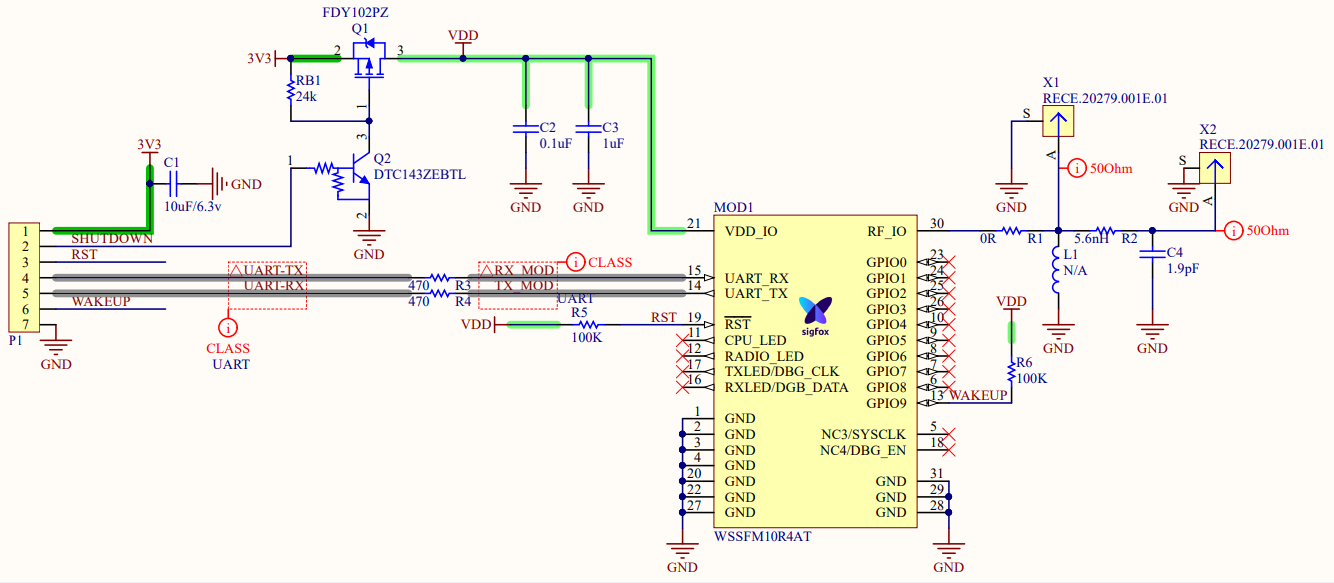
\includegraphics[scale=.45]{./Figures/SIGFOX_SCH.PNG}
	\caption{Esquemático módulo Sigfox.}
	\label{fig:SIGFOX_SCH}
\end{figure}

\subsubsection{Modulo Lora}
El módulo para la comunicación LoRa, es fabricado por la empresa  Microchip Technology.
\begin{itemize}
    \item  RN2903 \protect\footnotemark  clase A.
    \item Opera en la banda de frecuencia de 915 MHz
    \item modulación FSK, GFSK.
    \item 1.3 uA en modo \textit{sleep}.
    \item Potencia de Transmisión ajustable hasta 18.5 dBm.
\end{itemize}
\footnotetext{\url{http://ww1.microchip.com/downloads/en/DeviceDoc/50002390E.pdf}}

En la figura \ref{fig:lORA_SCH} se observa el diagrama esquemático del hardware asociado al módulo LoRa.

\begin{figure}[h]
	\centering
	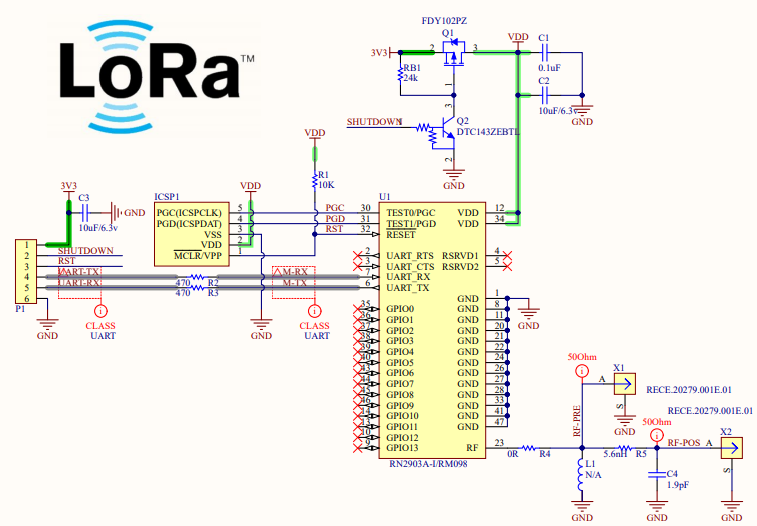
\includegraphics[scale=.55]{./Figures/lORA_SCH.PNG}
	\caption{Esquemático módulo LoRa.}
	\label{fig:lORA_SCH}
\end{figure}

\subsubsection{Entradas analógicas}

En la figura \ref{fig:inputanalog} se puede observar el diagrama esquemático de las entradas analógicas, los valores de las resistencias se escogieron de acuerdo a los niveles de tensión y de corriente de las entradas( 0-5VDC, 0-10VDC, 4-20mA) y el máximo voltaje permitido por el microcontrolador 3.3V. Todas las entradas analógicas tiene amplificadores en modo seguidor para acoplar impedancias y diodos TVS a la salida para garantizar los niveles de tensión máximo (3.3VDC).

\begin{figure}[h]
	\centering
	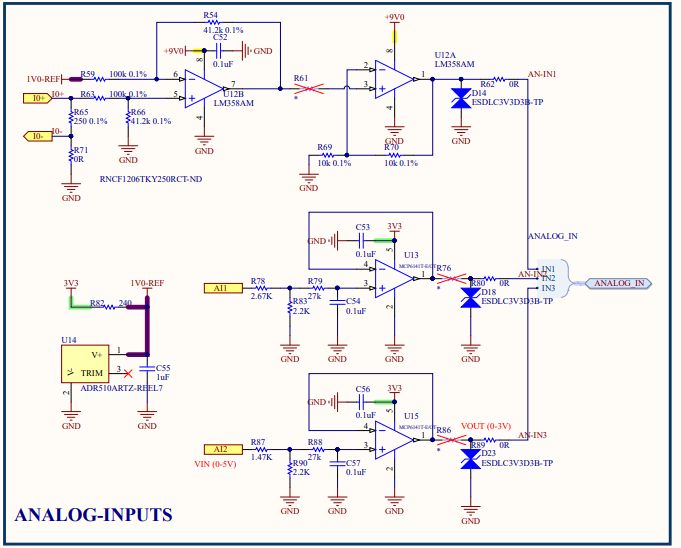
\includegraphics[scale=.65]{./Figures/inputanalog.PNG}
	\caption{Esquemático entradas analógicas.}
	\label{fig:inputanalog}
\end{figure}

\subsubsection{Entradas digitales}

En la figura \ref{fig:digitalinputs} se puede observar el diagrama esquemático de las entradas digitales, estas se encuentran optocopladas, aisladas y funcionan con niveles de voltaje entre 3.3VDC a 24VDC.

\begin{figure}[h]
	\centering
	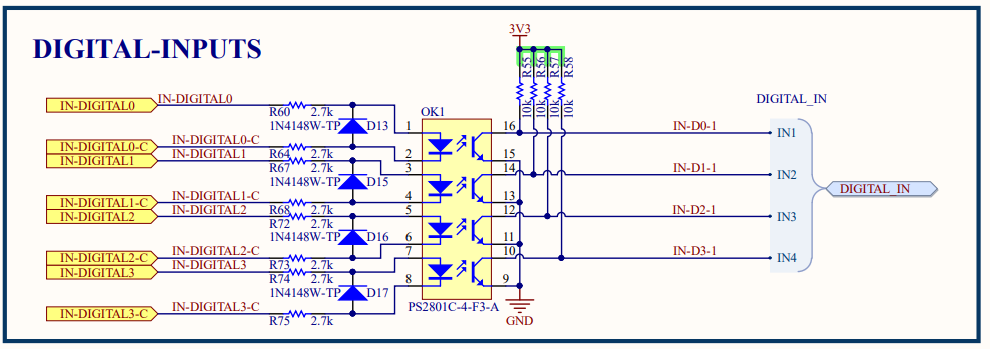
\includegraphics[scale=.45]{./Figures/digitalinputs.PNG}
	\caption{Esquemático entradas analógicas.}
	\label{fig:digitalinputs}
\end{figure}
% Se puede agregar código o pseudocódigo dentro de un entorno lstlisting con el siguiente código:

% \begin{verbatim}
% \begin{lstlisting}[caption= "un epígrafe descriptivo"]

% 	las líneas de código irían aquí...
	
% \end{lstlisting}
% \end{verbatim}

% A modo de ejemplo:

% \begin{lstlisting}[caption=Pseudocódigo del lazo principal de control.]  % Start your code-block

% #define MAX_SENSOR_NUMBER 3
% #define MAX_ALARM_NUMBER  6
% #define MAX_ACTUATOR_NUMBER 6

% uint32_t sensorValue[MAX_SENSOR_NUMBER];		
% FunctionalState alarmControl[MAX_ALARM_NUMBER];	//ENABLE or DISABLE
% state_t alarmState[MAX_ALARM_NUMBER];						//ON or OFF
% state_t actuatorState[MAX_ACTUATOR_NUMBER];			//ON or OFF

% void vControl() {

% 	initGlobalVariables();
	
% 	period = 500 ms;
		
% 	while(1) {

% 		ticks = xTaskGetTickCount();
		
% 		updateSensors();
		
% 		updateAlarms();
		
% 		controlActuators();
		
% 		vTaskDelayUntil(&ticks, period);
% 	}
% }
% \end{lstlisting}


%-------------
%
%--------------




\subsection{Selección de tecnologías a usar.}

\subsection{Sintonización y verificación de la antena.}

\subsection{Desarrollo de la capa de manejadores de dispsitivos(\textit{driver}).}

\subsection{Diseño del firmware}

\subsection{Implementación del firmware  y herramientas a usar.}



% Chapter Template

\chapter{Ensayos y Resultados} % Main chapter title

\label{Chapter4} % Change X to a consecutive number; for referencing this chapter elsewhere, use \ref{ChapterX}

%----------------------------------------------------------------------------------------
%	SECTION 1
%----------------------------------------------------------------------------------------

En esta sección se presentan los ensayos realizados, los resultados obtenidos y el análisis correspondiente.

\section{Dispositivos desarrollados}
En la figura \ref{fig:MainBoaard} se puede observar el resultado del diseño de la tarjeta. Esta se encuentra armada con los módulos insertables Sigfox y LoRa y fue sometida a diferentes ensayos indicados en la sección \ref{sec:pruebasHW} 

\begin{figure}[H]
	\centering
	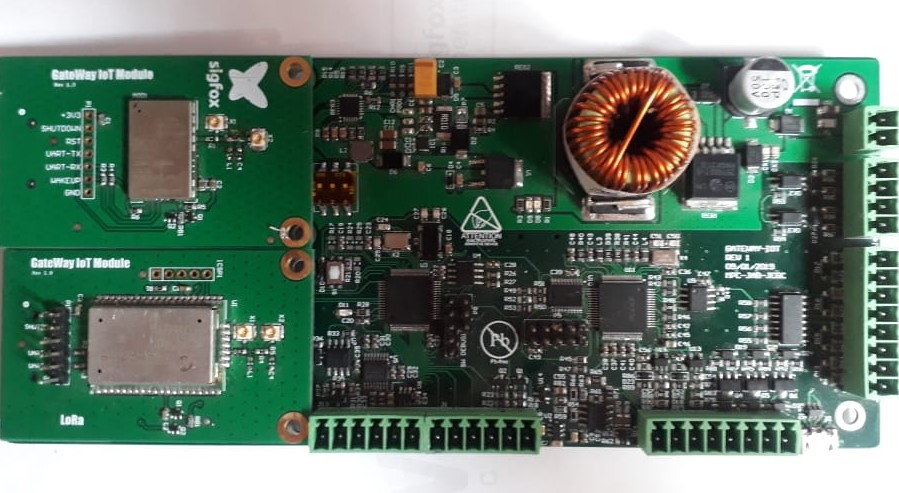
\includegraphics[scale=.45]{./Figures/MainBoardCompleta.jpeg}
	\caption{Tarjeta principal armada con los módulos Sifox y LoRa.}
	\label{fig:MainBoaard}
\end{figure}


\section{Pruebas de hardware sobre el prototipo} \label{sec:pruebasHW}
A la tarjeta se le hicieron pruebas individuales de hardware:
\begin{itemize}
    \item Cortos y continuidades.
    \item Voltaje en la linea de alimentación.
    \item Test visual comparado con el plano de ensamble, (ver figura
    \ref{fig:Planoensamble}.)
\end{itemize}

\begin{figure}[H]
	\centering
	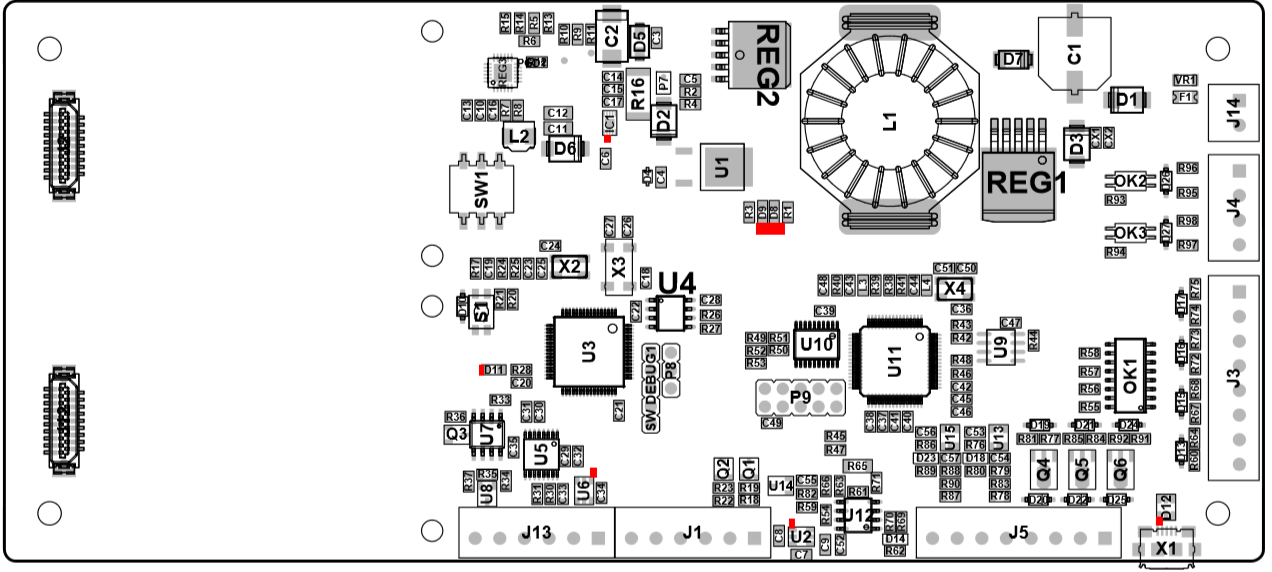
\includegraphics[scale=.45]{./Figures/Planoensamble.PNG}
	\caption{Plano de ensamble tarjeta principal.}
	\label{fig:Planoensamble}
\end{figure}

\section{Resultados de sintonización y verificación de la antena Sigfox}
En la ecuación \ref{eq:Impedancia2} y \ref{eq:Impedancia3} se pueden observar los valores de la impedancia y RL medidos con el VNA para una frecuencia de 915.516625 MHz.

En la figura \ref{fig:tunnigsigfoxchart} se puede observar el resultado de la verificación de la antena con el VNA, donde el marcador se encuentra muy cerca al origen de la carta de Smith y al eje real. Lo ideal en la sintonización es que el valor de la resistencia se acerque a \SI{50}{\ohm} y el valor de la reactancia (parte imaginaria \textit{j} de la ecuación \ref{eq:Impedancia2}) sea lo mas cercano a \SI{0}{\ohm} para garantizar la mejor eficiencia y la menor reflexión posible.

En la figura \ref{fig:tunnigsigfox5} se puede observar los resultados de la curva de perdidas de retorno. Esta deja evidenciar que tiene un ancho de banda de aproximadamente 125 KHz, el cual se mide a partir de -10dB\citep{AntenaSigFox2016}.


\begin{equation}
	\label{eq:Impedancia2}
	Z = 37.5\SI{}{\ohm} - j*4.7\SI{}{\ohm}
\end{equation}
\begin{equation}
	\label{eq:Impedancia3}
    RL = -16.35 dB
\end{equation}

\begin{figure}[H]
	\centering
	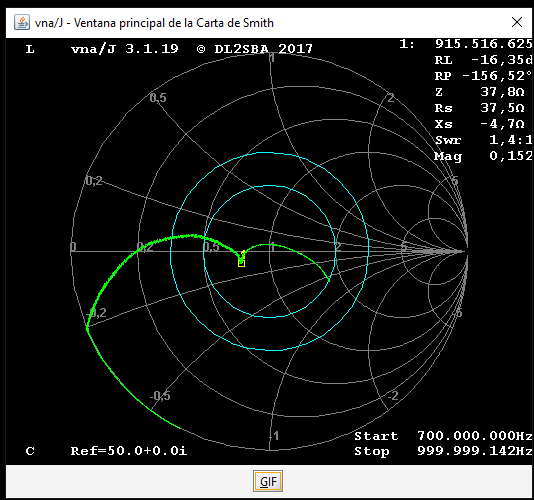
\includegraphics[scale=.7]{./Figures/tunnigsigfoxchart.png}
	\caption{Carta de Smith 915 MHz.}
	\label{fig:tunnigsigfoxchart}
\end{figure}

\begin{figure}[H]
	\centering
	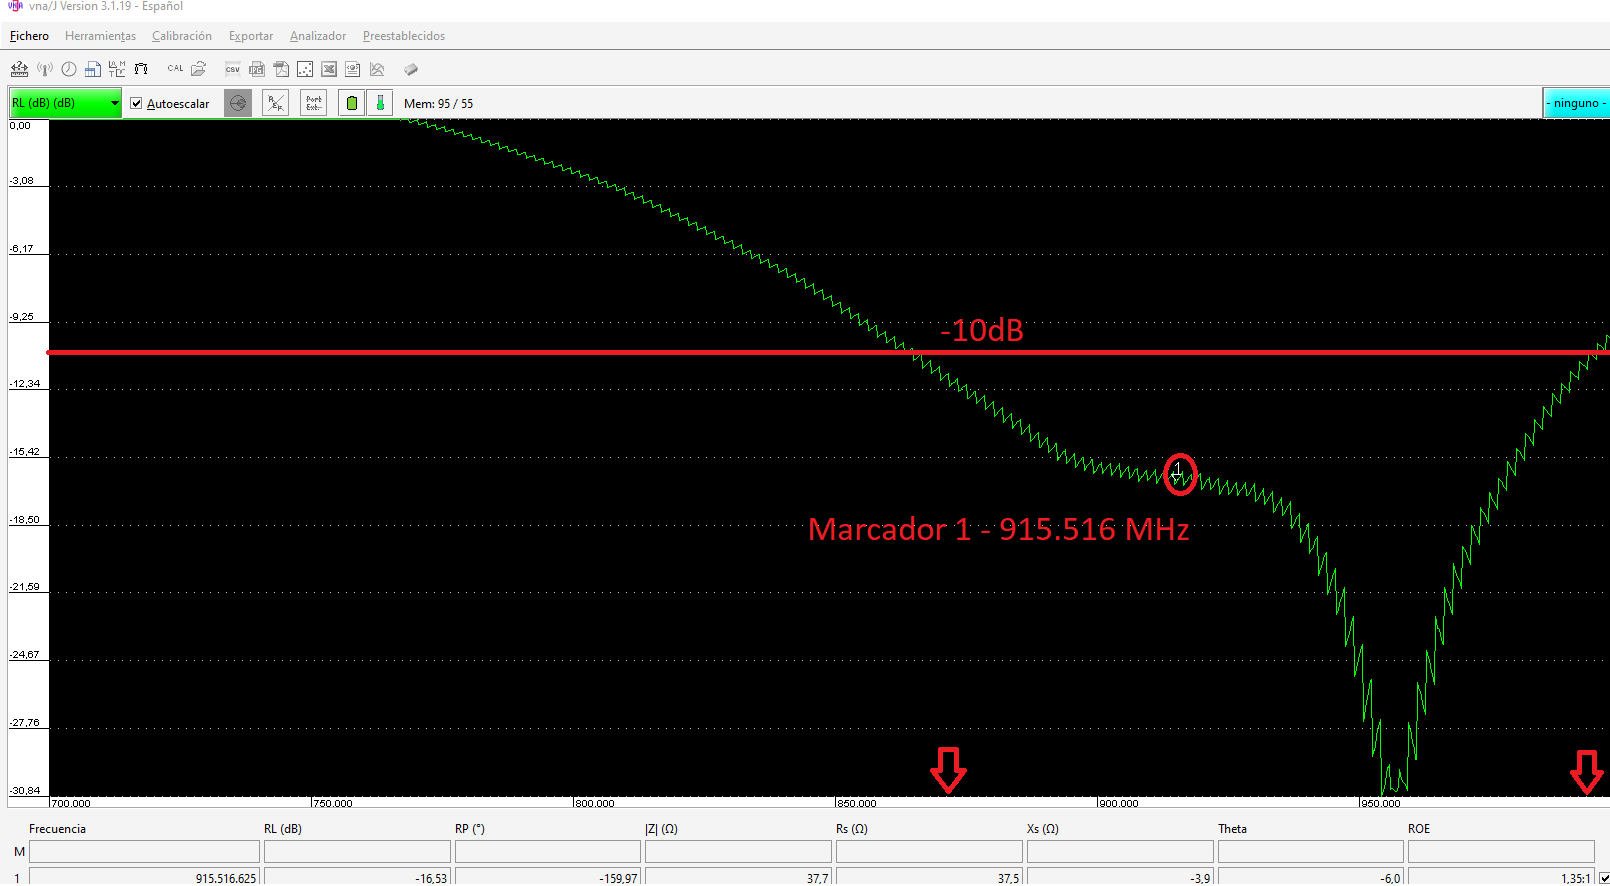
\includegraphics[scale=.35]{./Figures/tunnigsigfox5.png}
	\caption{Perdidas de retorno a 915 MHz.}
	\label{fig:tunnigsigfox5}
\end{figure}


%  Este valor de impedancia se encuentra muy cercano al eje real (37.5\SI{}{\ohm}). Entre mas cercano al eje real  y el valor de la reactancia X sea lo mas cercano a 0\SI{}{\ohm} habrán menos perdidos por reflexión. 


\section{Resultados de pruebas funcionales sobre  los módulos}

Los módulos Sigfox y LoRa se probaron individualmente, enviándole comandos AT y comandos MAC respectivamente. Con esto se verificó la correcta funcionalidad del dispositivo.
%y la verificación de consumos de corriente en modo \textit{Sleep}. 

% \begin{figure}[H]
% 	\centering
% %	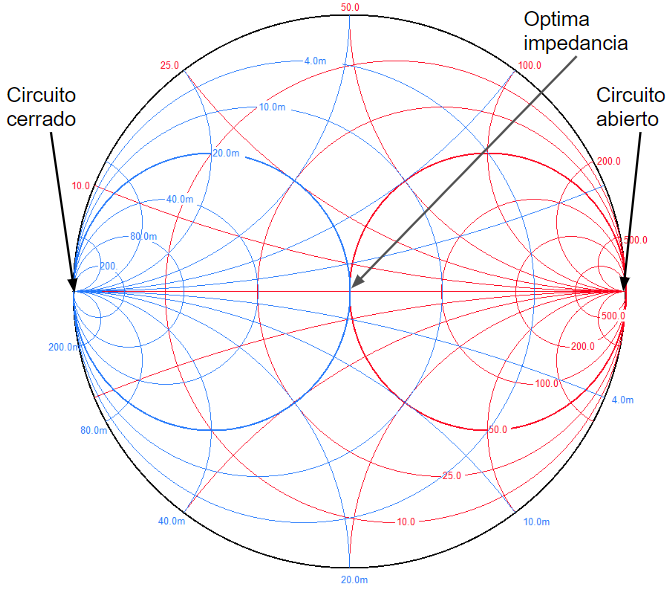
\includegraphics[scale=.45]{./Figures/CartaSmith.png}
% 	\caption{Consumo de corriente modulo Wisol - Sigfox.}
% 	\label{fig:ConsumoWisol}
% \end{figure}

% \begin{figure}[H]
% 	\centering
% %	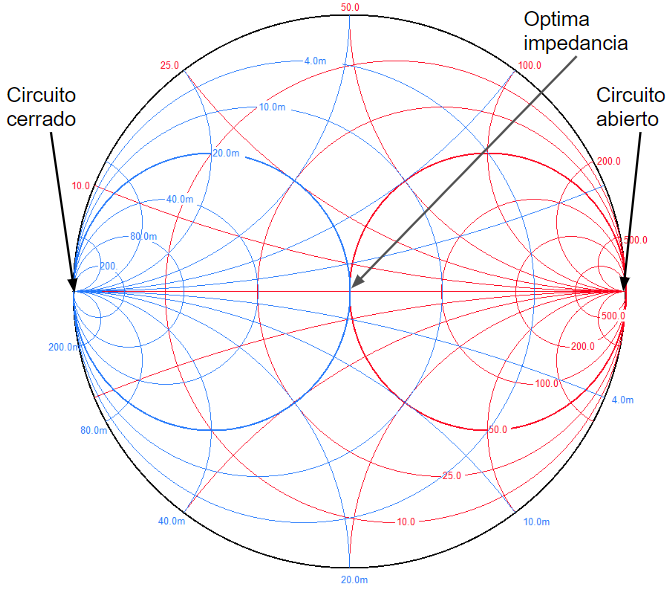
\includegraphics[scale=.45]{./Figures/CartaSmith.png}
% 	\caption{Consumo de corriente modulo RN2903 - LoRaWAN.}
% 	\label{fig:ConsumoLoraWAN}
% \end{figure}
\subsubsection{Resultados de las pruebas de transmisión de Sigfox}
Para la verificación de las transmisiones se uso el \textit{Back-end} Sigfox para la visualización de los paquetes de datos enviados.

En la figura \ref{fig:COMANDOSATSIGFOX} se pueden observar los comandos enviados al modulo Sigfox. En la figura \ref{fig:tRANSMISIONsIGFOX} se puede observar el mensaje de prueba visto en la plataforma de Sigfox. También se visualiza la cantidad (15) de estaciones bases que vieron el dispositivo y la cantidad de reenvíos (\textit{frames}), en 9 de 15 antenas se recibieron 3 de 3 paquetes enviados, por defecto Sigfox  envía tres \textit{frames} en cada transmisión y cada antena los recibe dependiendo de lo alejado que se encuentre el dispositivo de la estación base.

\begin{figure}[H]
	\centering
	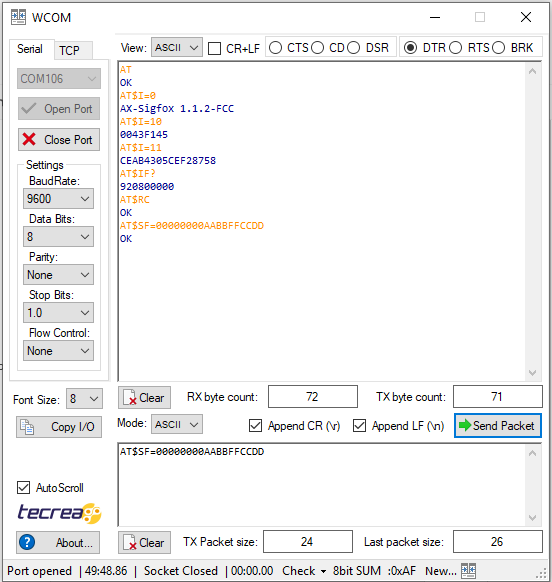
\includegraphics[scale=.5]{./Figures/COMANDOSATSIGFOX.PNG}
	\caption{Comandos enviados al módulo Wisol-Sigfox.}
	\label{fig:COMANDOSATSIGFOX}
\end{figure}
\begin{figure}[H]
	\centering
	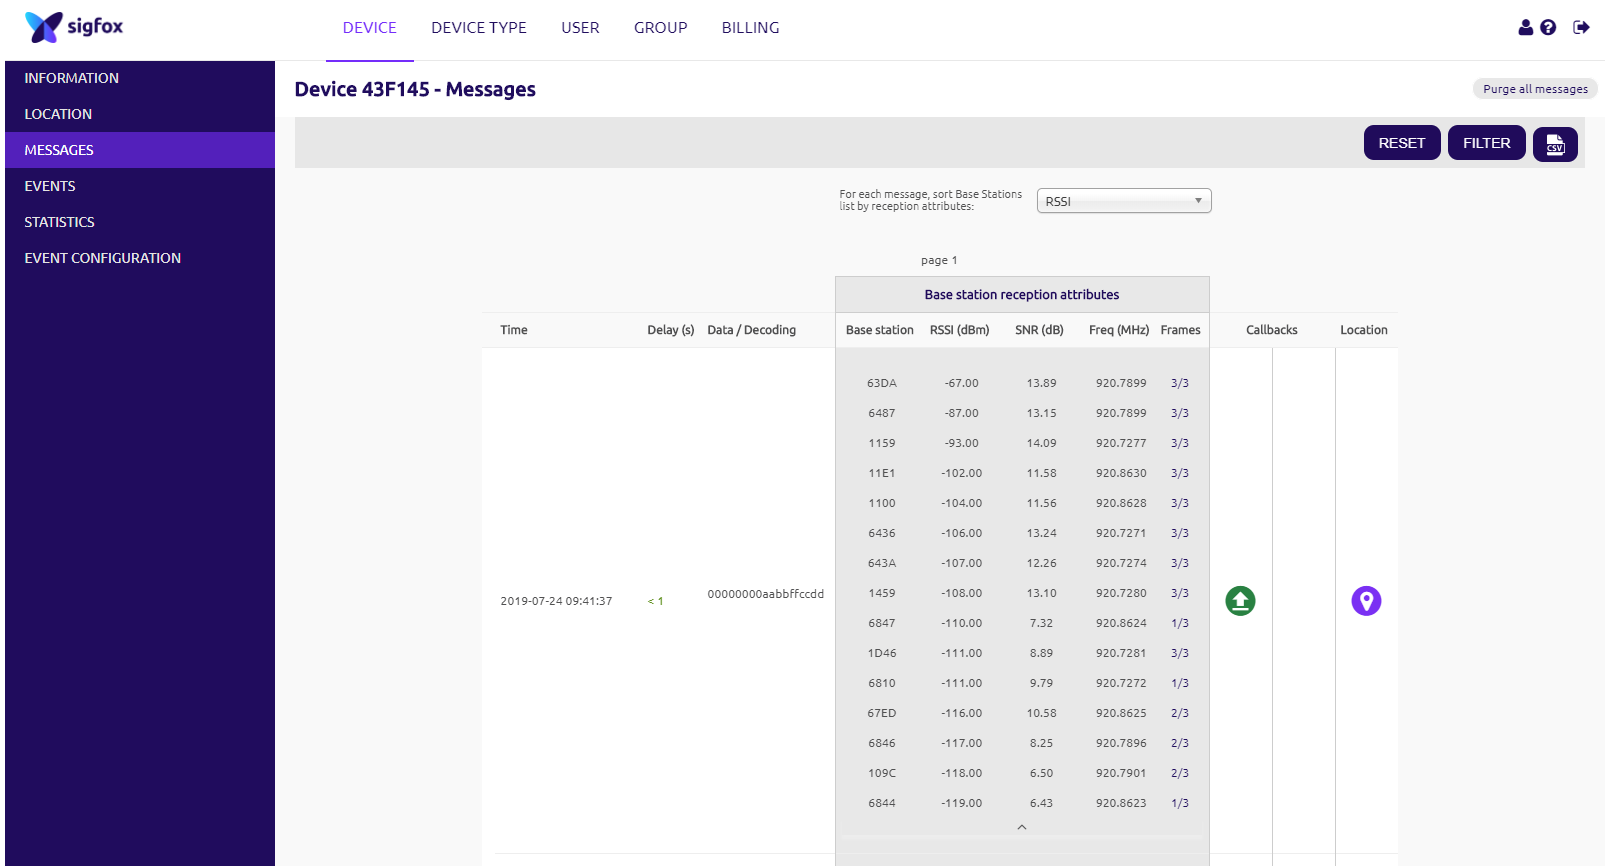
\includegraphics[scale=.35]{./Figures/tRANSMISIONsIGFOX.PNG}
	\caption{Prueba de transmisiones de mensajes de subida Sigfox.}
	\label{fig:tRANSMISIONsIGFOX}
\end{figure}

El dispositivo se alejo 10 Km del lugar de donde inicialmente se realizaron las transmisiones. En la figura \ref{fig:AntenasSigfoxAlejada} se puede observar que la cantidad (8 a 10) de estaciones base que vieron el dispositivo.
\begin{figure}[H]
	\centering
	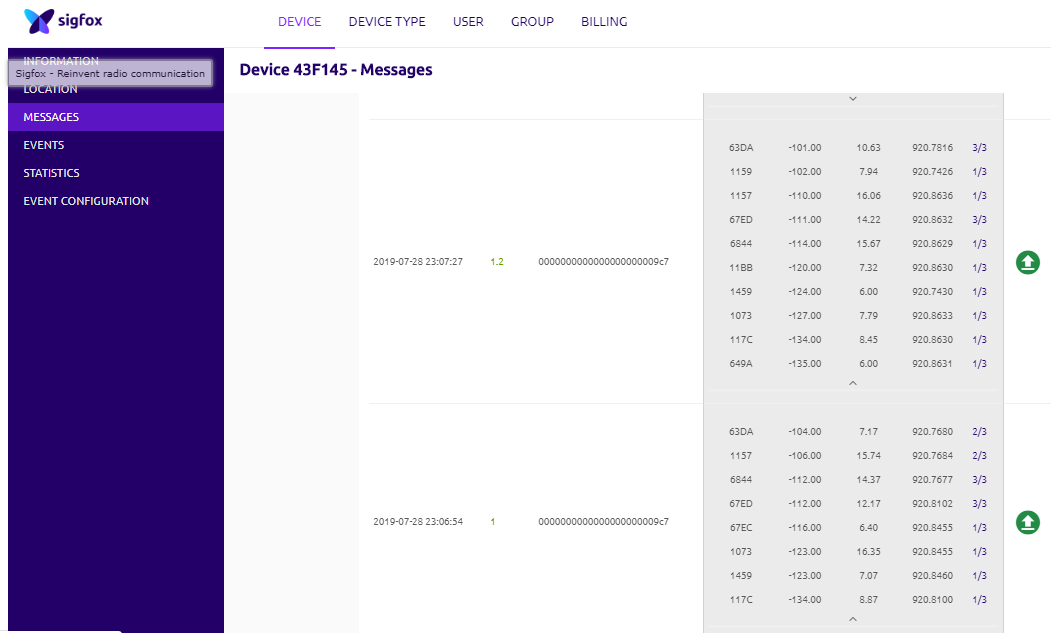
\includegraphics[scale=.45]{./Figures/AntenasSigfoxAlejada.PNG}
	\caption{Transmisiones de mensajes Sigfox a 10Km de distancia.}
	\label{fig:AntenasSigfoxAlejada}
\end{figure}

\subsubsection{Resultados de las pruebas de transmisión de LoRaWAN}

En la figura \ref{fig:ComandMacLora} se pueden observar los comandos enviados al modulo LoRaWAN. Para la verificación de las transmisiones de loRaWAN se usó el servidor \textit{the things network} para la visualización de los paquetes de datos enviados (ver figura \ref{fig:Datalorawantest}).


\begin{figure}[H]
	\centering
	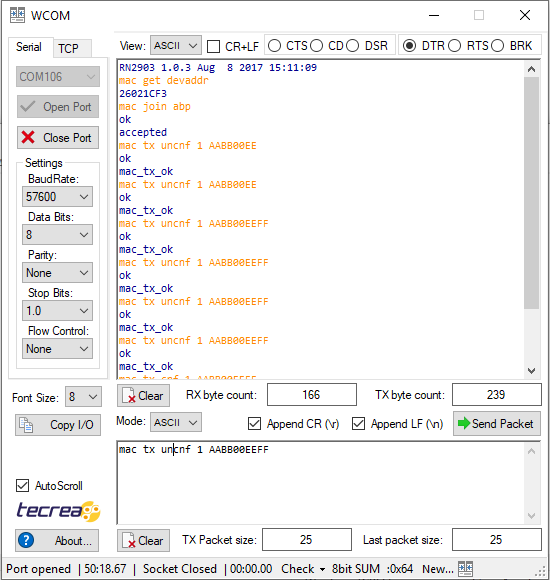
\includegraphics[scale=.45]{./Figures/ComandMacLora.PNG}
	\caption{Comandos enviados al módulo LoRaWAN.}
	\label{fig:ComandMacLora}
\end{figure}
\begin{figure}[H]
	\centering
	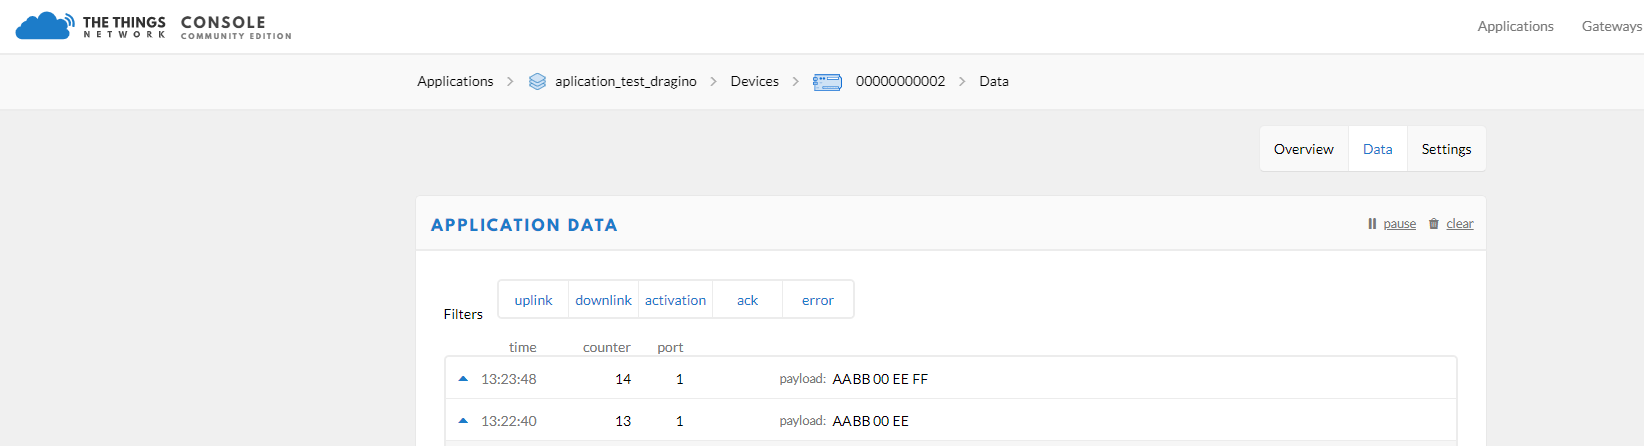
\includegraphics[scale=.35]{./Figures/Datalorawantest.PNG}
	\caption{Prueba de transmision de mensajes con LoRaWAN.}
	\label{fig:Datalorawantest}
\end{figure}

En la figura \ref{fig:LoraTX_corto} se puede observar que de 156 mensajes transmitidos con el dispositivo a una distancia menor a 1m del gateway. Solo 6 mensajes fueron recibidos por el servidor.
\begin{figure}[H]
	\centering
	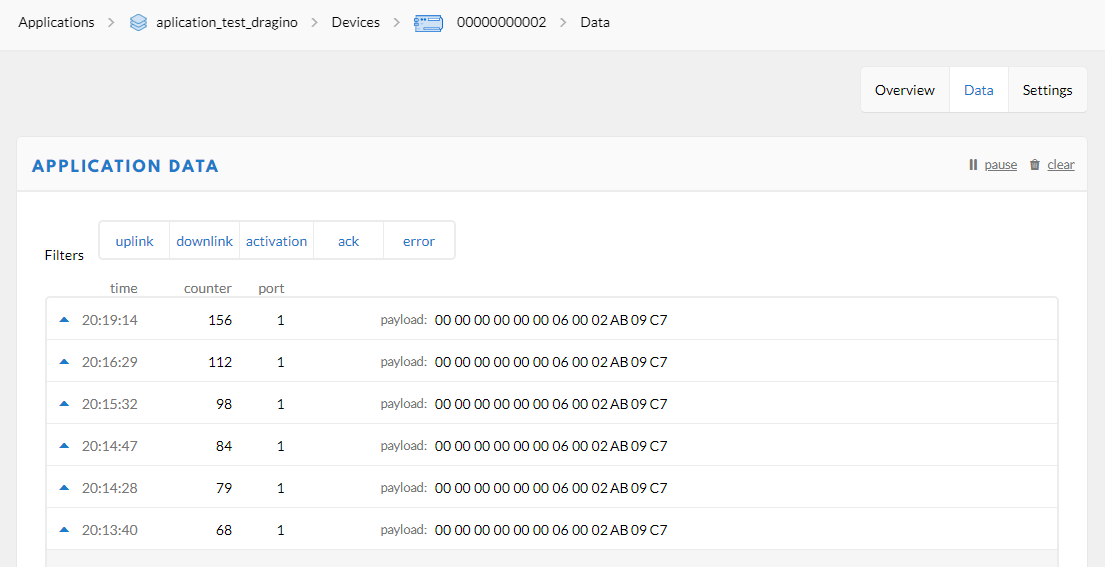
\includegraphics[scale=.5]{./Figures/LoraTX_corto.PNG}
	\caption{Cuantificación de mensajes enviados con LoRaWAN.}
	\label{fig:LoraTX_corto}
\end{figure}
%\footnotetext{\url{https://www.thethingsnetwork.org/}}

\section{Pruebas de consumo de energía}
Los módulos LoRaWAN y Sigfox trabajan bajo redes LPWAN, por lo que el consumo debe ser lo más bajo posible. Esto debido a que en las aplicaciones se busca que los dispositivos finales tengan una durabilidad de muchos años. En la tabla \ref{tab:ConsumosTabla} se pueden observar los datos de los consumos usados.

\begin{table}[h]
	\centering
	\caption[Consumos]{Medición de consumos energéticos Sigfox y LoRaWAN }
	\begin{tabular}{l c c}    
		\toprule
		\textbf{ \textit{Modo} } & \textbf{Sigfox} & \textbf{LoRaWAN} \\
		\midrule
		Normal	    &$\mathrm{0.53 mA}$ 	&$\mathrm{6.71 mA}$  \\	
		\textit{Sleep}	            & $\mathrm{0.3 \mu{A}}$     & $\mathrm{6.4 \mu{A}}$\\
		\bottomrule
		\hline
	\end{tabular}
	\label{tab:ConsumosTabla}
\end{table}


El consumo energético del modulo Sigfox WWSFM11R2D se puede observar en la figura \ref{fig:Consumo_SigNormal} y \ref{fig:ConsumoSigSleep}. 
\begin{figure}[H]
	\centering
	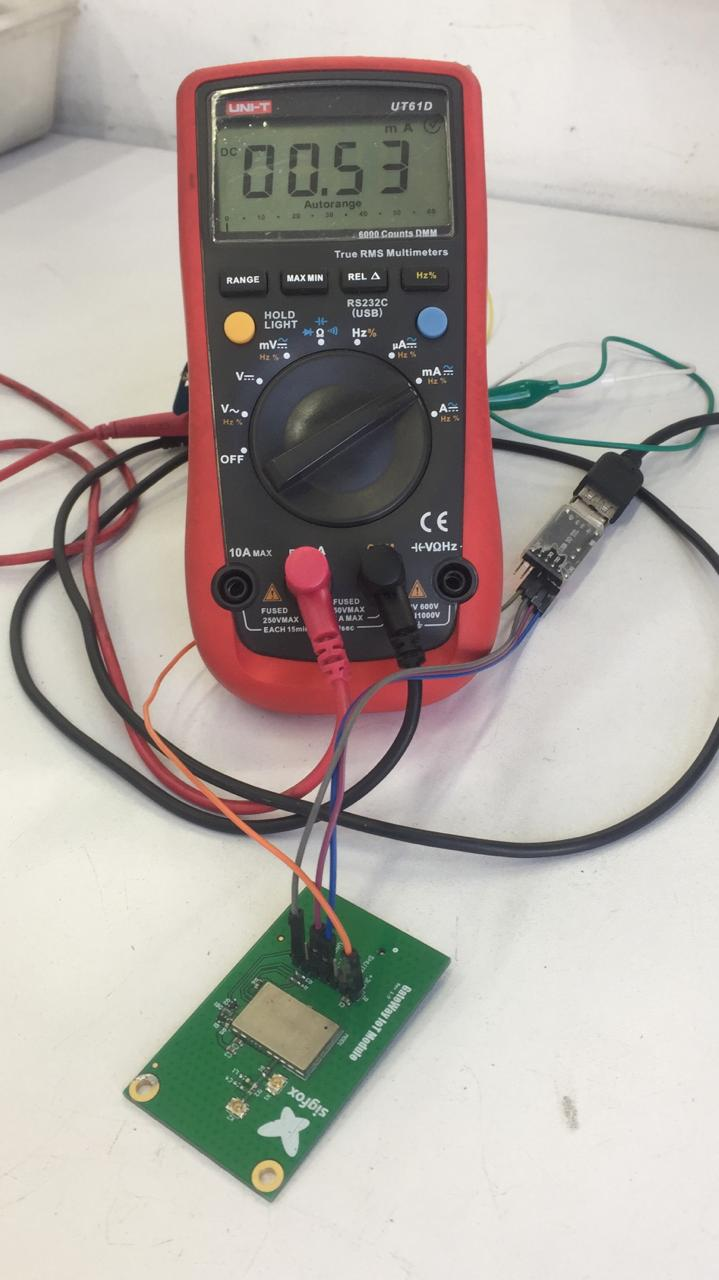
\includegraphics[scale=.15]{./Figures/Consumo_SigNormal.jpeg}
	\caption{Consumo de WWSFM11R2D en funcionamiento normal.}
	\label{fig:Consumo_SigNormal}
\end{figure}

\begin{figure}[H]
	\centering
	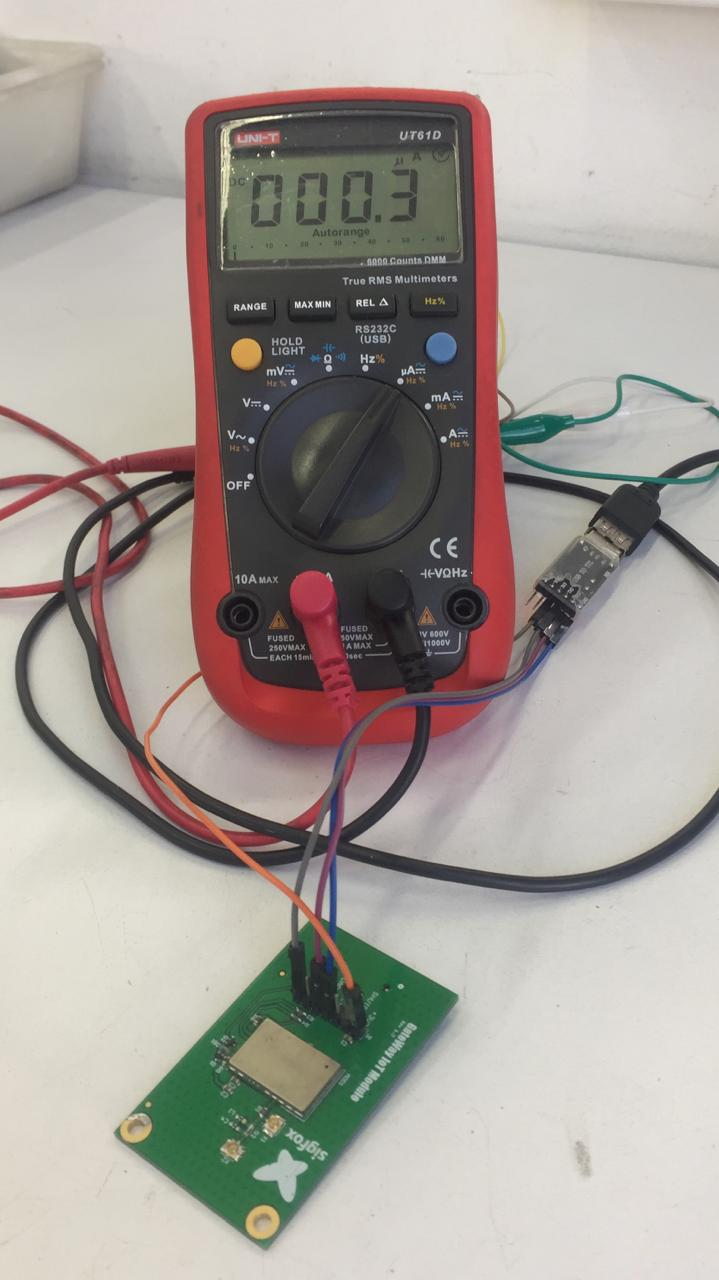
\includegraphics[scale=.15]{./Figures/ConsumoSigSleep.jpeg}
	\caption{Consumo de WWSFM11R2D en modo \textit{sleep}}
	\label{fig:ConsumoSigSleep}
\end{figure}

El consumo energético del modulo LoRaWAN se puede observar en la figura \ref{fig:ConsumoLoraNormal} y \ref{fig:ConsumoLoraSleep}. 

\begin{figure}[H]
	\centering
	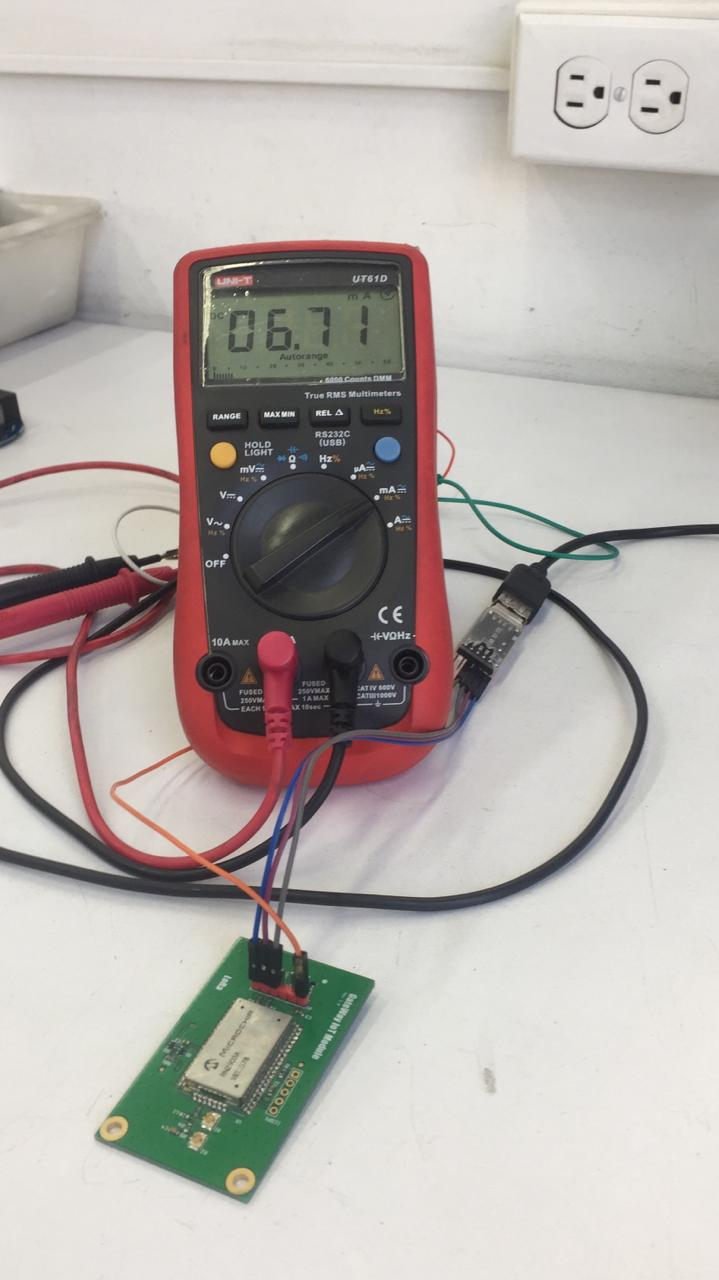
\includegraphics[scale=.15]{./Figures/ConsumoLoraNormal.jpeg}
	\caption{Consumo de RN2903 en funcionamiento normal.}
	\label{fig:ConsumoLoraNormal}
\end{figure}

\begin{figure}[H]
	\centering
	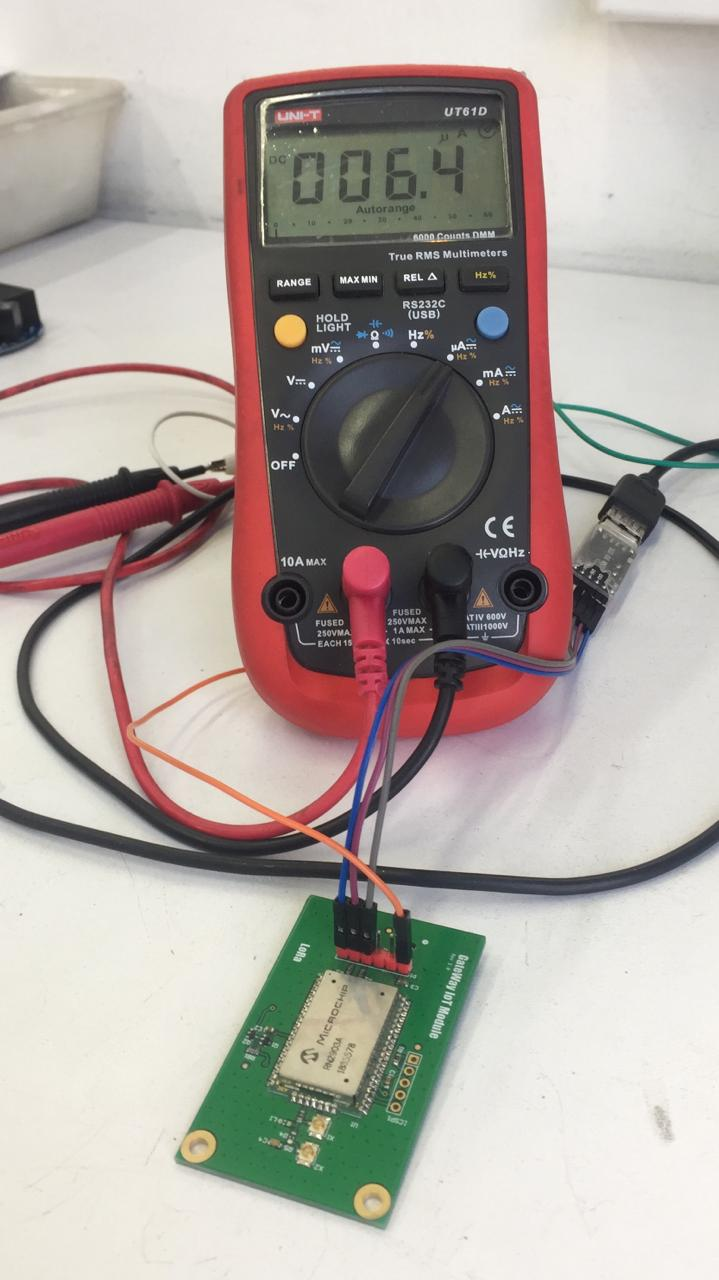
\includegraphics[scale=.15]{./Figures/ConsumoLoraSleep.jpeg}
	\caption{Consumo de RN2903 en modo \textit{sleep}}
	\label{fig:ConsumoLoraSleep}
\end{figure}

La medición de corriente en los módulos deja evidenciar que mientras se encuentra en modo de funcionamiento el consumo es alto, sin embargo cuando se les envía el comando para entrar en modo de bajo consumo la corriente baja considerablemente al orden de $\mu{A}$.


\section{Pruebas de integración}
Para las pruebas de integración se contó con :
\begin{itemize}
    \item Acceso remoto al servidor de Sigfox y LoRaWAN. 
    \item Acceso remoto a  la plataforma xxxx para no visualizar las señales en crudo.
    \item Acceso físico a los dispositivos embebidos
    \item Terminal serial WCOM desarrollada por Tecrea SAS.
    \item Multimetro UNI-T ut61D con resolución de hasta 100 nA.
    \item Acceso a consola serial de la tarjeta principal.
\end{itemize}

En la figura \ref{fig:IntegracionSL2} se puede observar la consola de depuracíon del dispositivo. Durante el proceso de pruebas permitió la visualización del estado interno de la aplicación embebida al mostrar los mensajes impresos por el firmware desarrollado. Se puede visualizar que el mensaje enviado es:

00 00 00 00 00 00 06 00 02 AB 09 c7 

Este se puede decodificar de acuerdo a la siguiente imagen \ref{fig:FRAME}, como cada canal analógico es de 12 bits, al valor de los canales ADC0, ADC1, ADC2 se les debe aplicar la formula \ref{eq:ADC} para obtener el resultado de 2.786 V, 4.5 V y 0 mA.

\begin{equation}
	\label{eq:ADC}
	VADCx = (ADCx -2340 ) / 58.5
\end{equation}

\begin{figure}[H]
	\centering
	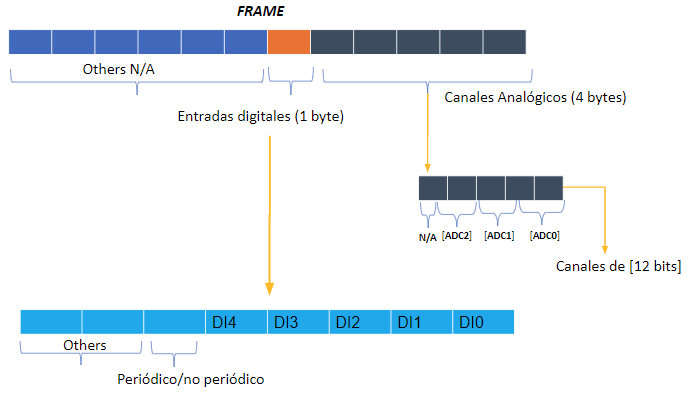
\includegraphics[scale=.6]{./Figures/FRAME.PNG}
	\caption{Codificación del paquete de datos.}
	\label{fig:FRAME}
\end{figure}

\begin{figure}[H]
	\centering
	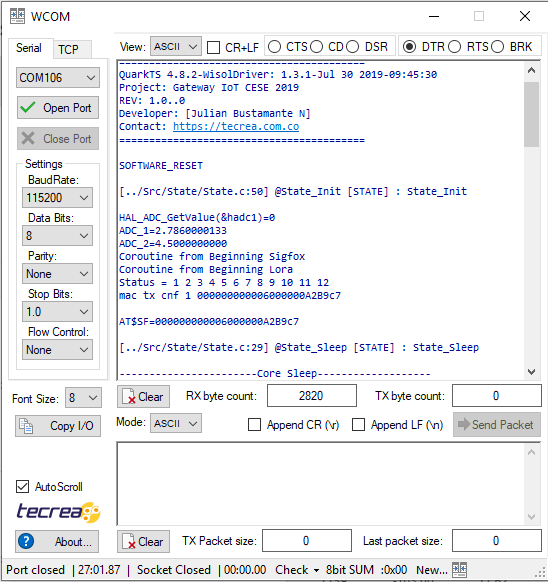
\includegraphics[scale=.6]{./Figures/IntegracionSL2.PNG}
	\caption{Consola de depuración del sistema embebido.}
	\label{fig:IntegracionSL2}
\end{figure}


En la figura \ref{fig:Ubidotsintegration} se puede observar la visualización del \textit{dashboard} con la medición de las variables en la plataforma Ubidots.

\begin{figure}[H]
	\centering
	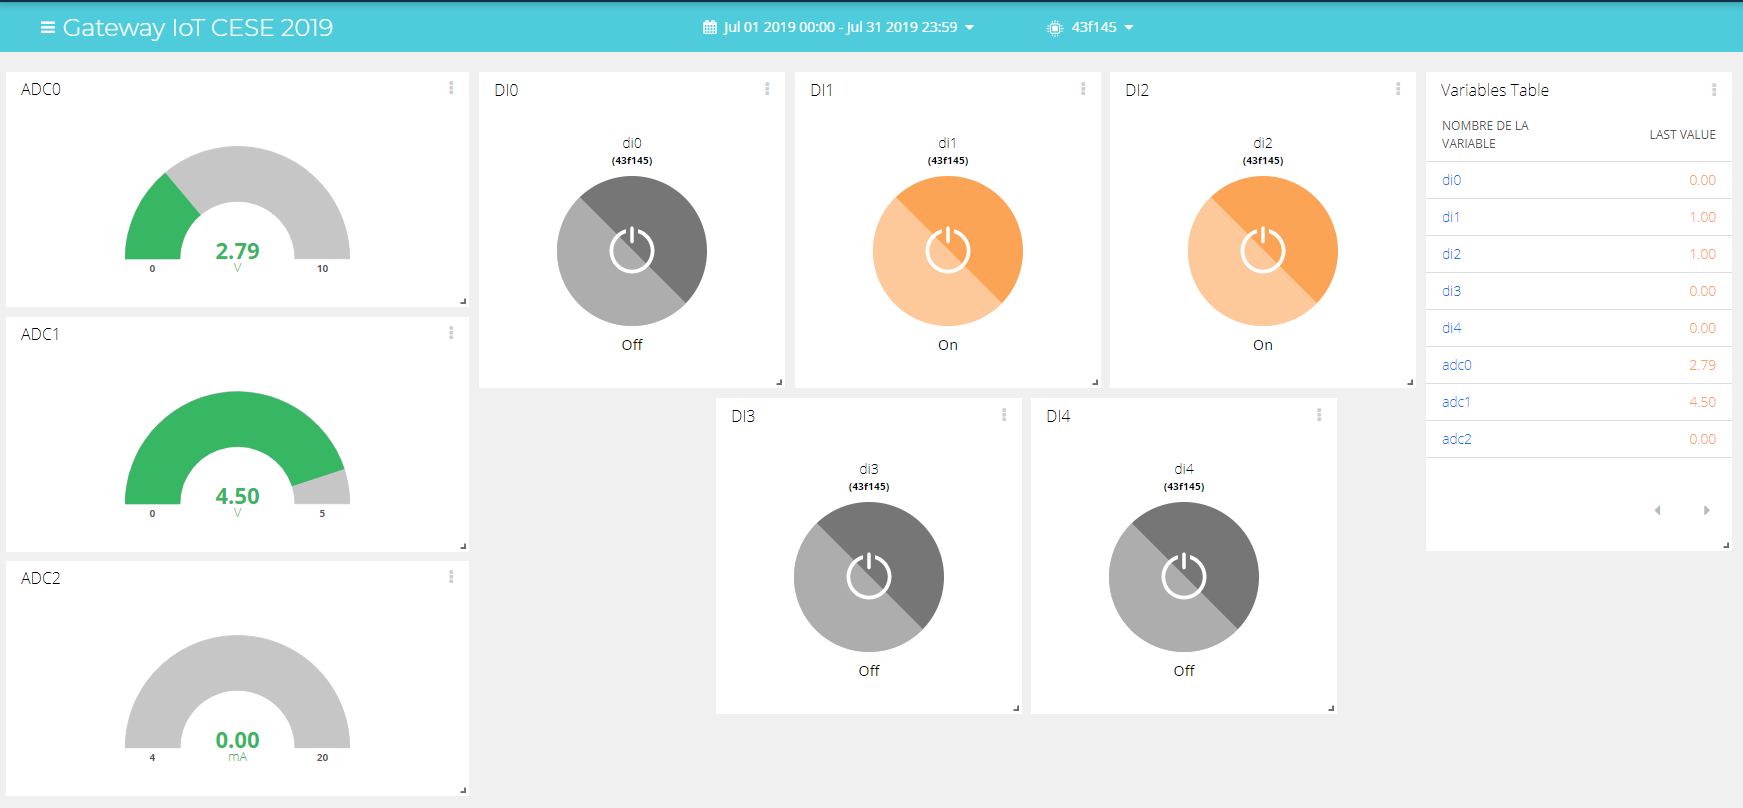
\includegraphics[scale=.3]{./Figures/Ubidotsintegration.PNG}
	\caption{Plataforma de integración.}
	\label{fig:Ubidotsintegration}
\end{figure}

%\section{Pruebas unitarias de manejadores de dispositivos (\textit{driver})}








 
% Chapter Template

\chapter{Conclusiones} % Main chapter title

\label{Chapter5} % Change X to a consecutive number; for referencing this chapter elsewhere, use \ref{ChapterX}


%----------------------------------------------------------------------------------------

%----------------------------------------------------------------------------------------
%	SECTION 1
%----------------------------------------------------------------------------------------

\section{Conclusiones generales }

La idea de esta sección es resaltar cuáles son los principales aportes del trabajo realizado y cómo se podría continuar. Debe ser especialmente breve y concisa. Es buena idea usar un listado para enumerar los logros obtenidos.

%----------------------------------------------------------------------------------------
%	SECTION 2
%----------------------------------------------------------------------------------------
\section{Próximos pasos}

Acá se indica cómo se podría continuar el trabajo más adelante.
 

%----------------------------------------------------------------------------------------
%	CONTENIDO DE LA MEMORIA  - APÉNDICES
%----------------------------------------------------------------------------------------

\appendix % indicativo para indicarle a LaTeX los siguientes "capítulos" son apéndices

% Incluir los apéndices de la memoria como archivos separadas desde la carpeta Appendices
% Descomentar las líneas a medida que se escriben los apéndices

%% Appendix A

\chapter{Appendix Title Here} % Main appendix title

\label{AppendixA} % For referencing this appendix elsewhere, use \ref{AppendixA}

Write your Appendix content here.
%\include{Appendices/AppendixB}
%\include{Appendices/AppendixC}

%----------------------------------------------------------------------------------------
%	BIBLIOGRAPHY
%----------------------------------------------------------------------------------------

\Urlmuskip=0mu plus 1mu\relax
\raggedright
\printbibliography[heading=bibintoc]

%----------------------------------------------------------------------------------------

\end{document}  
